% ==================/// PHASES ///==================
\section{Phases }
% ==================/// PHASE 1 – TEXT ///==================
\begin{frame}{Phase 1: TF setup and perception}
	\small
	\textbf{Goal: Prepare clean TF data for simulation}
	\vspace{0.3cm}
	
	\begin{itemize}
		\item<1-> \textbf{Step 1 — Put tags on the map.}\\[0.05cm]
		We save where each AprilTag sits:
		\[
		T_{\text{world}}^{\text{tag}}
		\]
		This stays fixed for every next step.
		
		\item<2-> \textbf{Step 2 — Drive the robot once.}\\[0.05cm]
		The simulator gives the robot pose while it follows a smooth curve:
		\[
		T_{\text{world}}^{\text{camera\_link}}(t)
		\]
		
		\item<3-> \textbf{Step 3 — Use the real camera frame.}\\[0.05cm]
		We switch to the optical frame (how the camera really looks):
		\[
		T_{\text{world}}^{\text{camera\_optical}}(t)
		=
		T_{\text{world}}^{\text{camera\_link}}(t)
		\cdot
		T_{\text{camera\_link}}^{\text{camera\_optical}}
		\]
		
		\item<4-> \textbf{Step 4 — Clean tag detections.}\\[0.05cm]
		From the map and pose we get, for each tag:
		\[
		T_{\text{camera\_optical}}^{\text{tag}}(t)
		\]
	
	\end{itemize}
\end{frame}

% ==================/// PHASE 1 – VISUAL ///==================
\begin{frame}{Phase 1: TF setup and perception — Visual}
	\centering
	\vspace{0.3cm}
	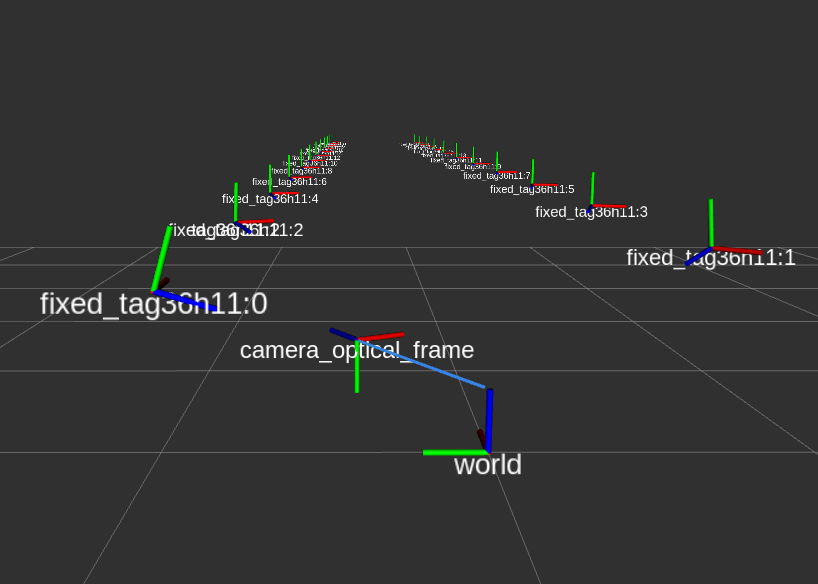
\includegraphics[height=0.75\textheight]{assets/TF.png}\\
	{\tiny\textit{Fig. 4 — World, robot and camera frames}}
\end{frame}



% ==================/// PHASE 2 – TEXT ///==================
\begin{frame}{Phase 2: Simulation and dataset generation}
	\small
	\textbf{Goal: Create a realistic noisy dataset for testing}
	\vspace{0.3cm}
	
	\begin{itemize}
		\item<1-> \textbf{Step 1 — Simulate a clean path.}\\[0.05cm]
		We make a smooth curve and log the true pose:
		\[
		T_{\text{world}}^{\text{camera\_optical}}(t)
		\]
		
		\item<2-> \textbf{Step 2 — Compute perfect tag reads.}\\[0.05cm]
		For every tag and time we compute the clean detection:
		\[
		T_{\text{camera\_optical}}^{\text{tag}}(t)
		\]
		
		\item<3-> \textbf{Step 3 — Add noise like real life.}\\[0.05cm]
		We add Gaussian noise so readings look imperfect, like real sensors.
		
		\item<4-> \textbf{Step 4 — Save the dataset.}\\[0.05cm]
		For each time we save:
		\begin{itemize}
			\item the true pose $T_{\text{world}}^{\text{camera\_optical}}(t)$
			\item the noisy tag detections $T_{\text{camera\_optical}}^{\text{tag}}(t)$
		\end{itemize}
	\end{itemize}
\end{frame}



% ==================/// PHASE 2 – VISUAL 1 (RETO) ///==================
\begin{frame}{Phase 2: Visual — Straight trajectory with tags}
	\centering
	\vspace{0.2cm}
	
	\begin{columns}[T]
		\begin{column}{0.5\textwidth}
			\centering
			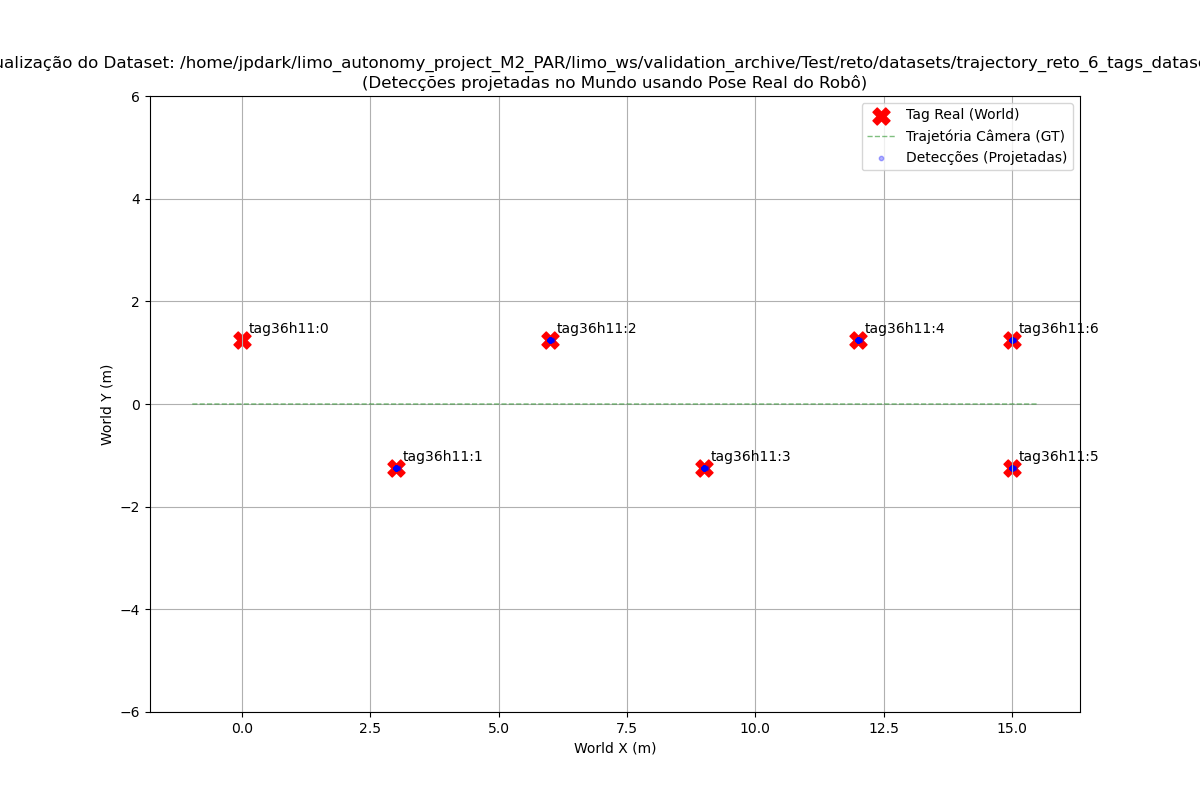
\includegraphics[width=\textwidth]{assets/datasets/trajectory_reto_6_tags_dataset_plot.png}\\[0.1cm]
			{\tiny Clean straight-path dataset (6 tags)}
		\end{column}
		
		\begin{column}{0.5\textwidth}
			\centering
			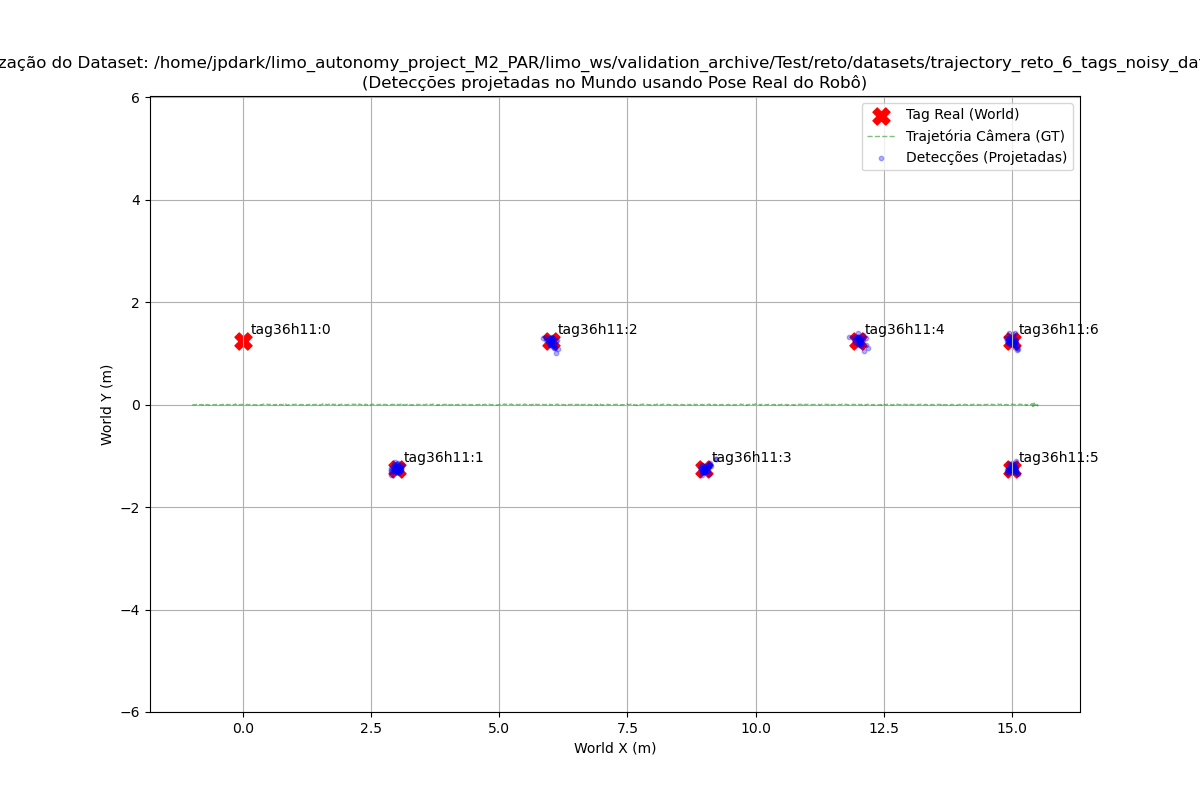
\includegraphics[width=\textwidth]{assets/datasets/trajectory_reto_6_tags_noisy_dataset_plot.png}\\[0.1cm]
			{\tiny Noisy straight-path dataset}
		\end{column}
	\end{columns}
	
	\vspace{0.15cm}
	{\tiny\textit{Fig. 5.1 — Straight trajectory: clean (left) and noisy (right)}}
\end{frame}



% ==================/// PHASE 2 – VISUAL 2 (S-CURVE 5 TAGS) ///==================
\begin{frame}{Phase 2: Visual — S-curve trajectory with 5 tags}
	\centering
	\vspace{0.2cm}
	
	\begin{columns}[T]
		\begin{column}{0.5\textwidth}
			\centering
			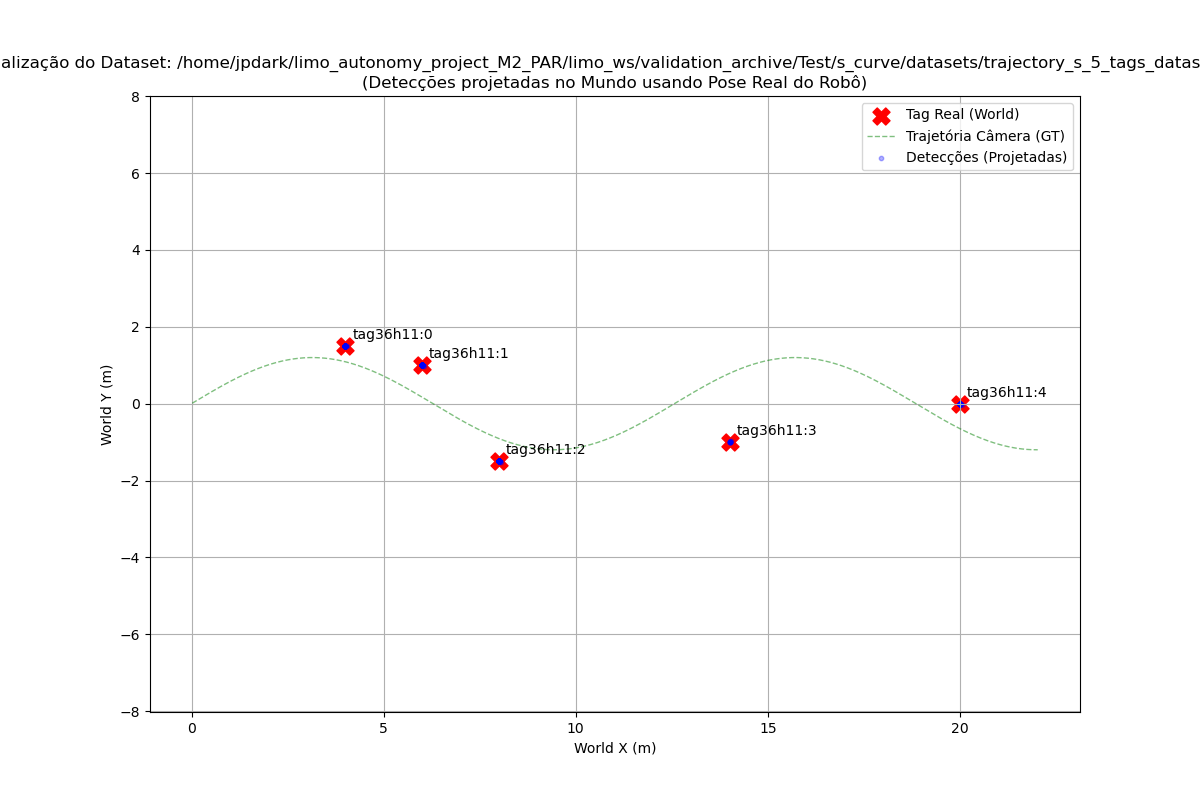
\includegraphics[width=\textwidth]{assets/datasets/trajectory1.png}\\[0.1cm]
			{\tiny Clean S-curve dataset (5 tags)}
		\end{column}
		
		\begin{column}{0.5\textwidth}
			\centering
			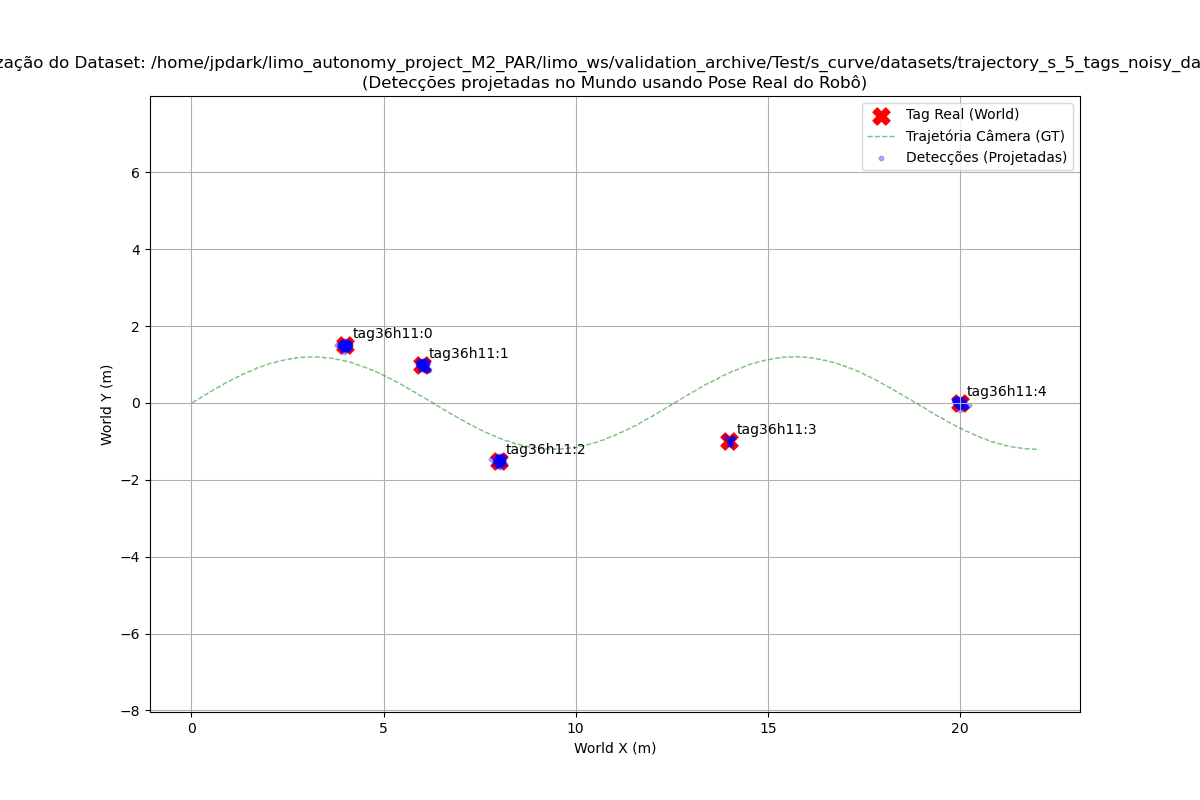
\includegraphics[width=\textwidth]{assets/datasets/trajectory2.png}\\[0.1cm]
			{\tiny Noisy S-curve dataset (5 tags)}
		\end{column}
	\end{columns}
	
	\vspace{0.15cm}
	{\tiny\textit{Fig. 5.2 — S-curve with 5 tags: clean (left) and noisy (right)}}
\end{frame}



% ==================/// PHASE 2 – VISUAL 3 (S-CURVE MANY TAGS) ///==================
\begin{frame}{Phase 2: Visual — Dense S-curve trajectory}
	\centering
	\vspace{0.2cm}
	
	\begin{columns}[T]
		\begin{column}{0.5\textwidth}
			\centering
			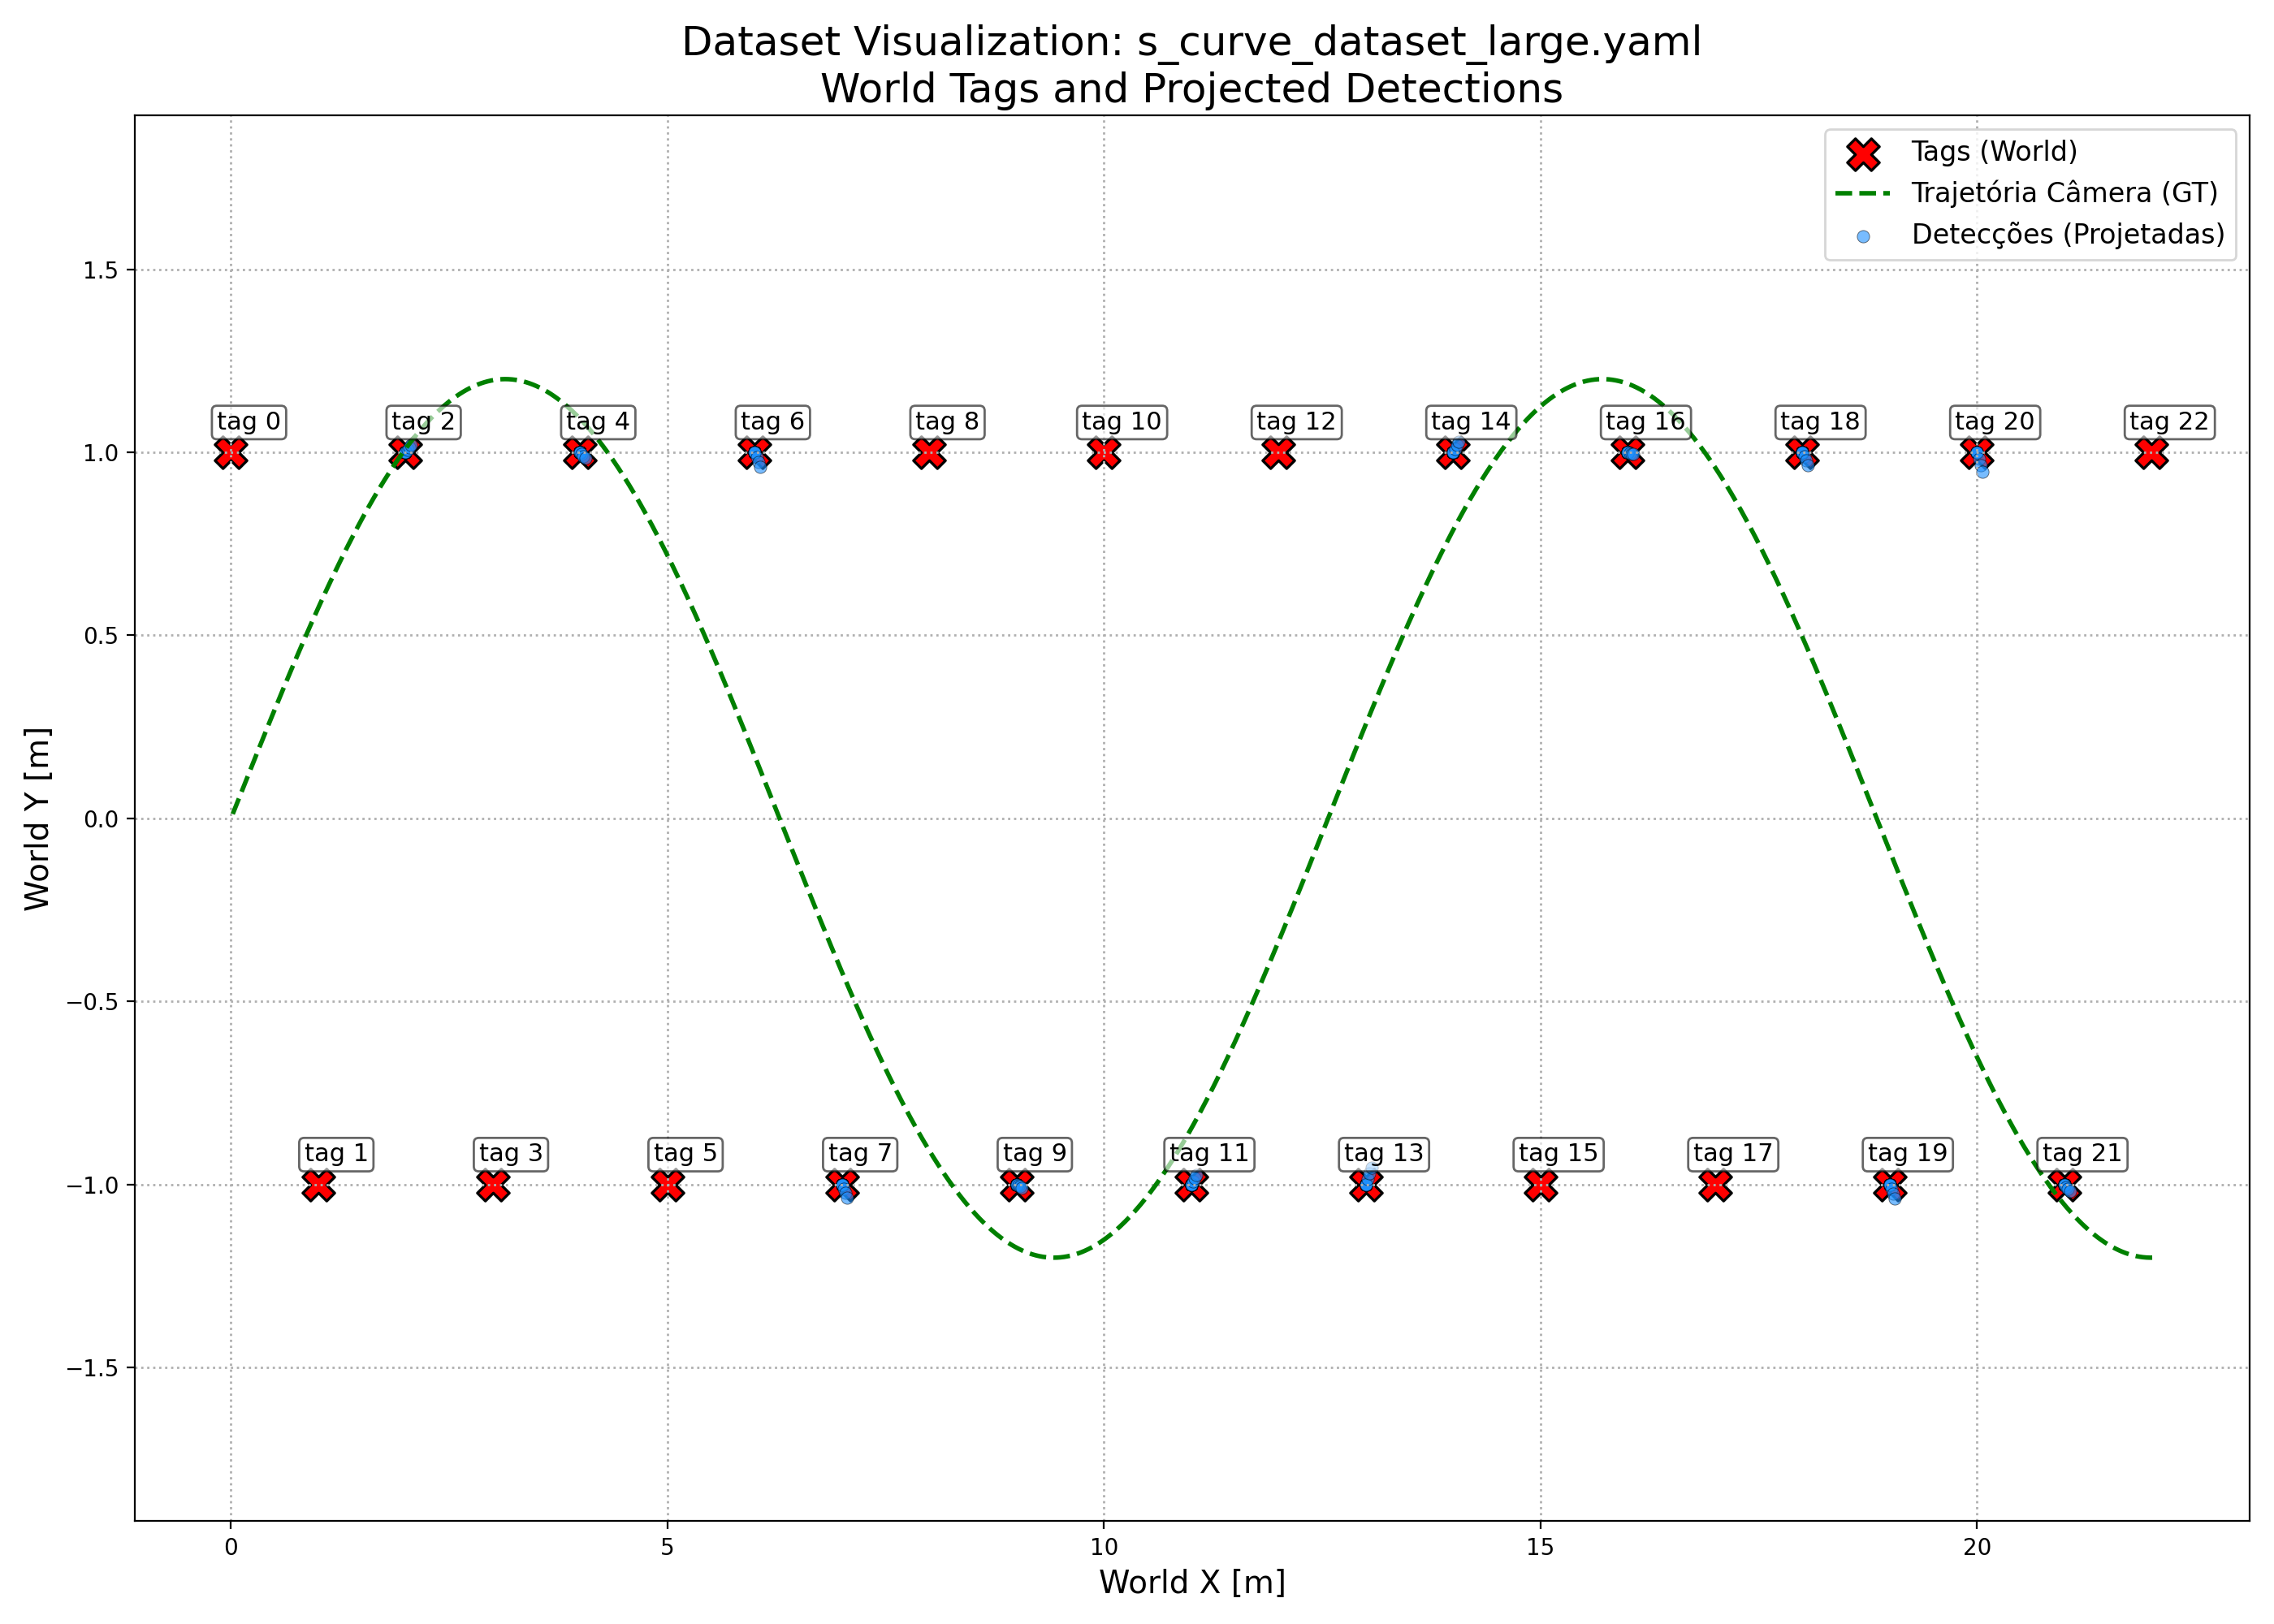
\includegraphics[width=\textwidth]{assets/s_curve_dataset_large_plot_big.png}\\[0.1cm]
			{\tiny Clean S-curve dataset (dense tags)}
		\end{column}
		
		\begin{column}{0.5\textwidth}
			\centering
			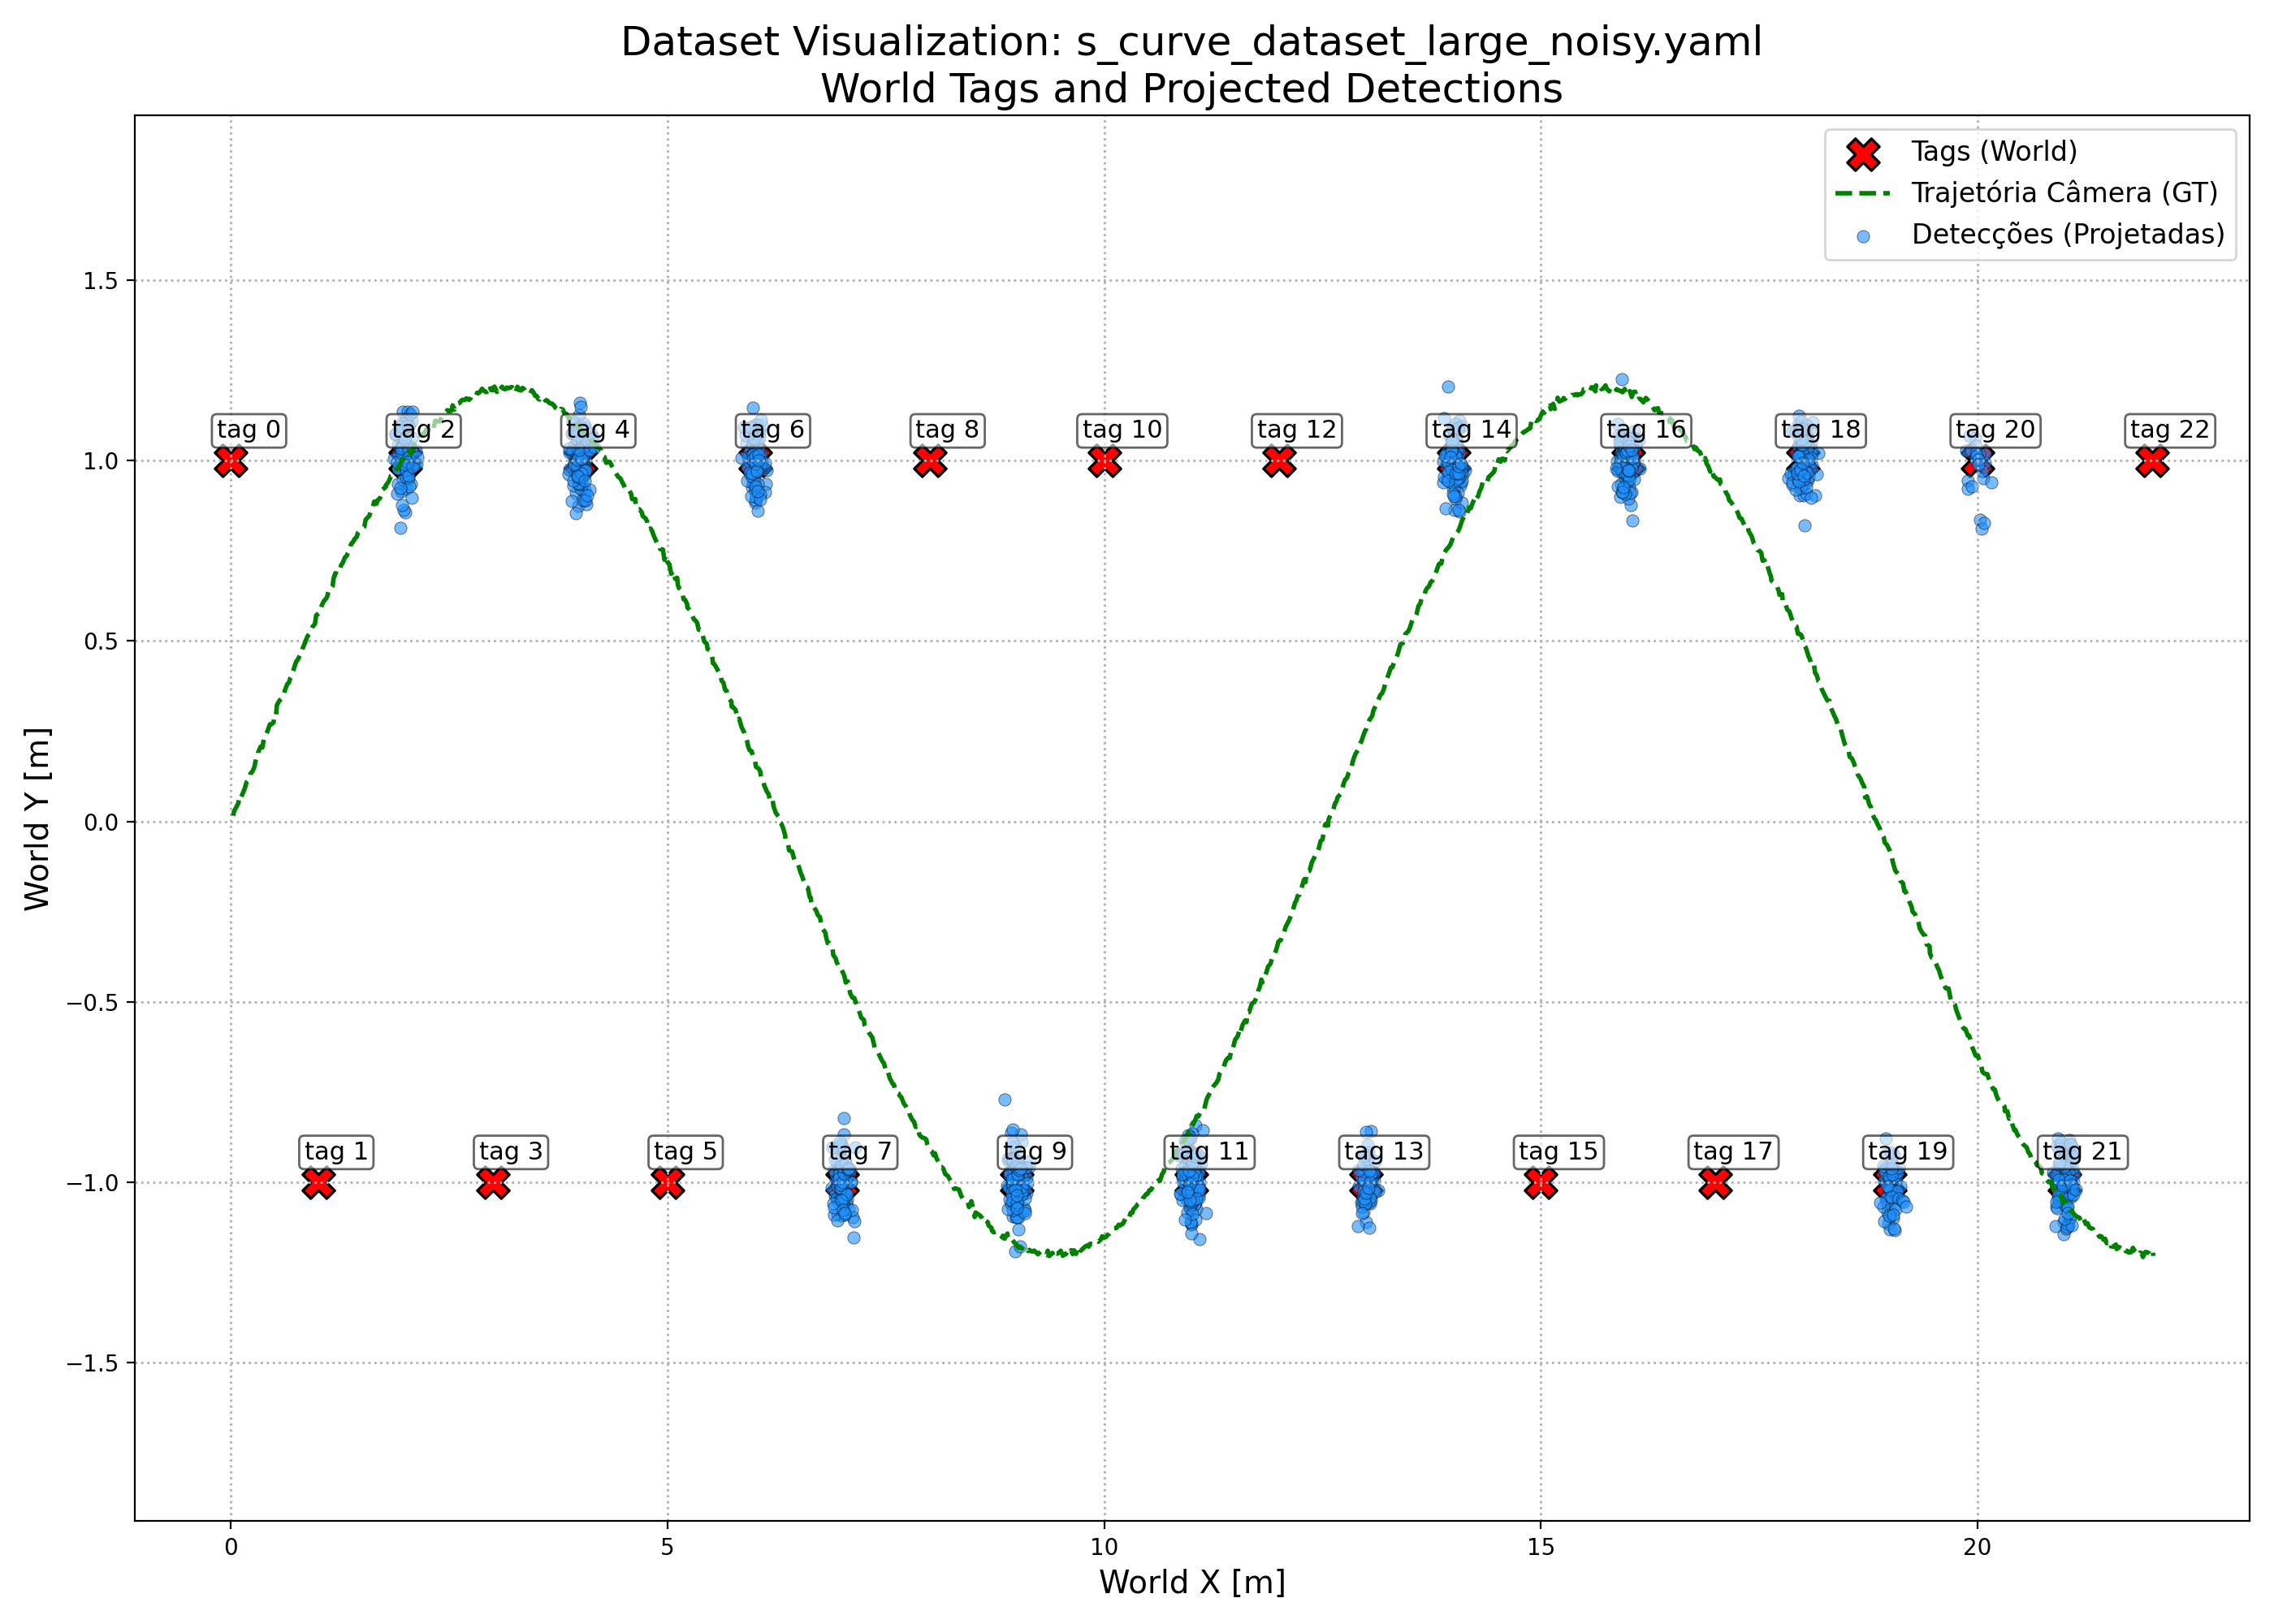
\includegraphics[width=\textwidth]{assets/s_curve_dataset_large_noisy_plot_big.png}\\[0.1cm]
			{\tiny Noisy S-curve dataset (dense tags)}
		\end{column}
	\end{columns}
	
	\vspace{0.15cm}
	{\tiny\textit{Fig. 5.3 — S-curve with many tags: clean (left) and noisy (right)}}
\end{frame}

% ==================/// PHASE 3 ///==================
\begin{frame}{Phase 3: Trajectory Optimization \& Recovery}
            \textbf{Goal: Fix drift with a simple optimizer}
            \vspace{0.5cm}
            \begin{itemize}
                \item<1-> \textbf{Path recovery:}  
                Align the noisy run with the taught path.

                \item<2-> \textbf{Pose graph:}  
                Reduce error between waypoints and simple constraints.

                \item<3-> \textbf{Drift fix:}  
                Auto-correct rotation and position drift.
            \end{itemize}
\end{frame}









\begin{frame}{Recovery the Optimal Path Sinusoidal Trajectory} % <-- Título mantido
    \centering
    \begin{columns}
        

        \begin{column}{0.5\textwidth}
            \centering
            % Sua imagem de recuperação
            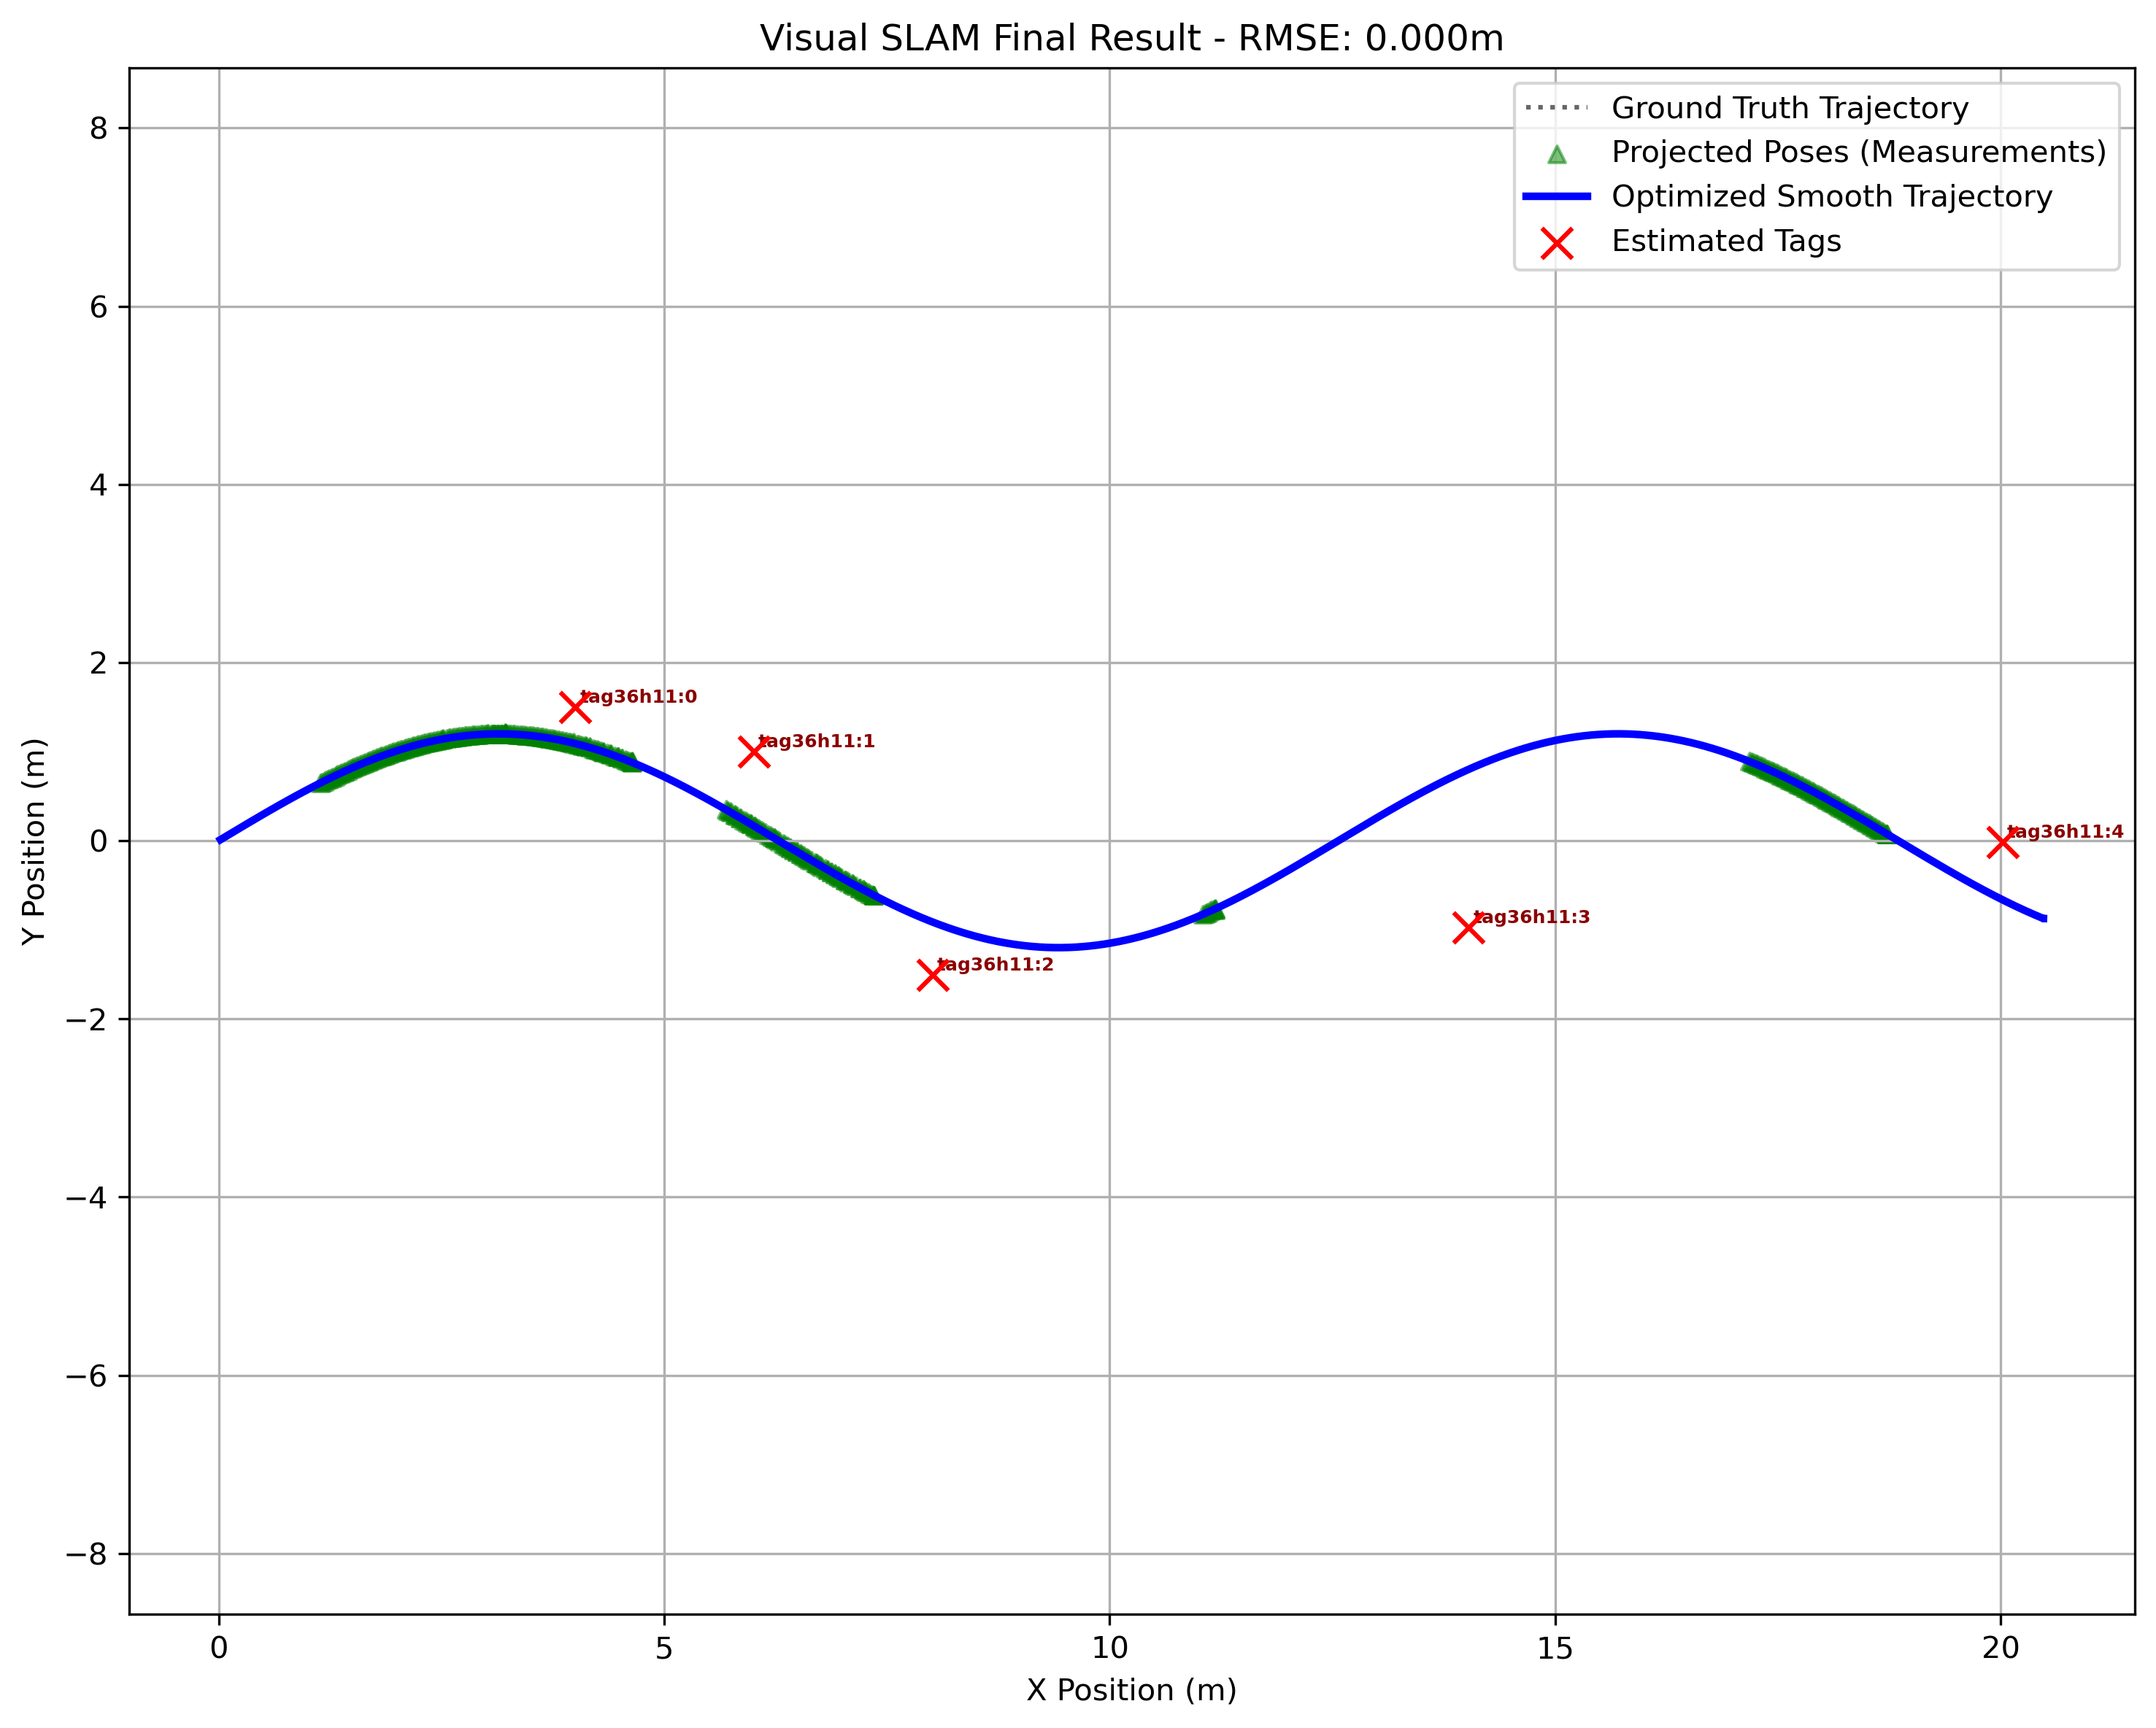
\includegraphics[width=\textwidth]{assets/s_final_graph.png}
            \vspace{0.2cm}
            {\small\textit{Fig. 7.2 — Trajectory Recovery via Optimization}}
        \end{column}

        % COLUNA ESQUERDA: Dados Ruidosos
        \begin{column}{0.5\textwidth}
            \centering
            % Imagem do dataset ruidoso da Phase 2
            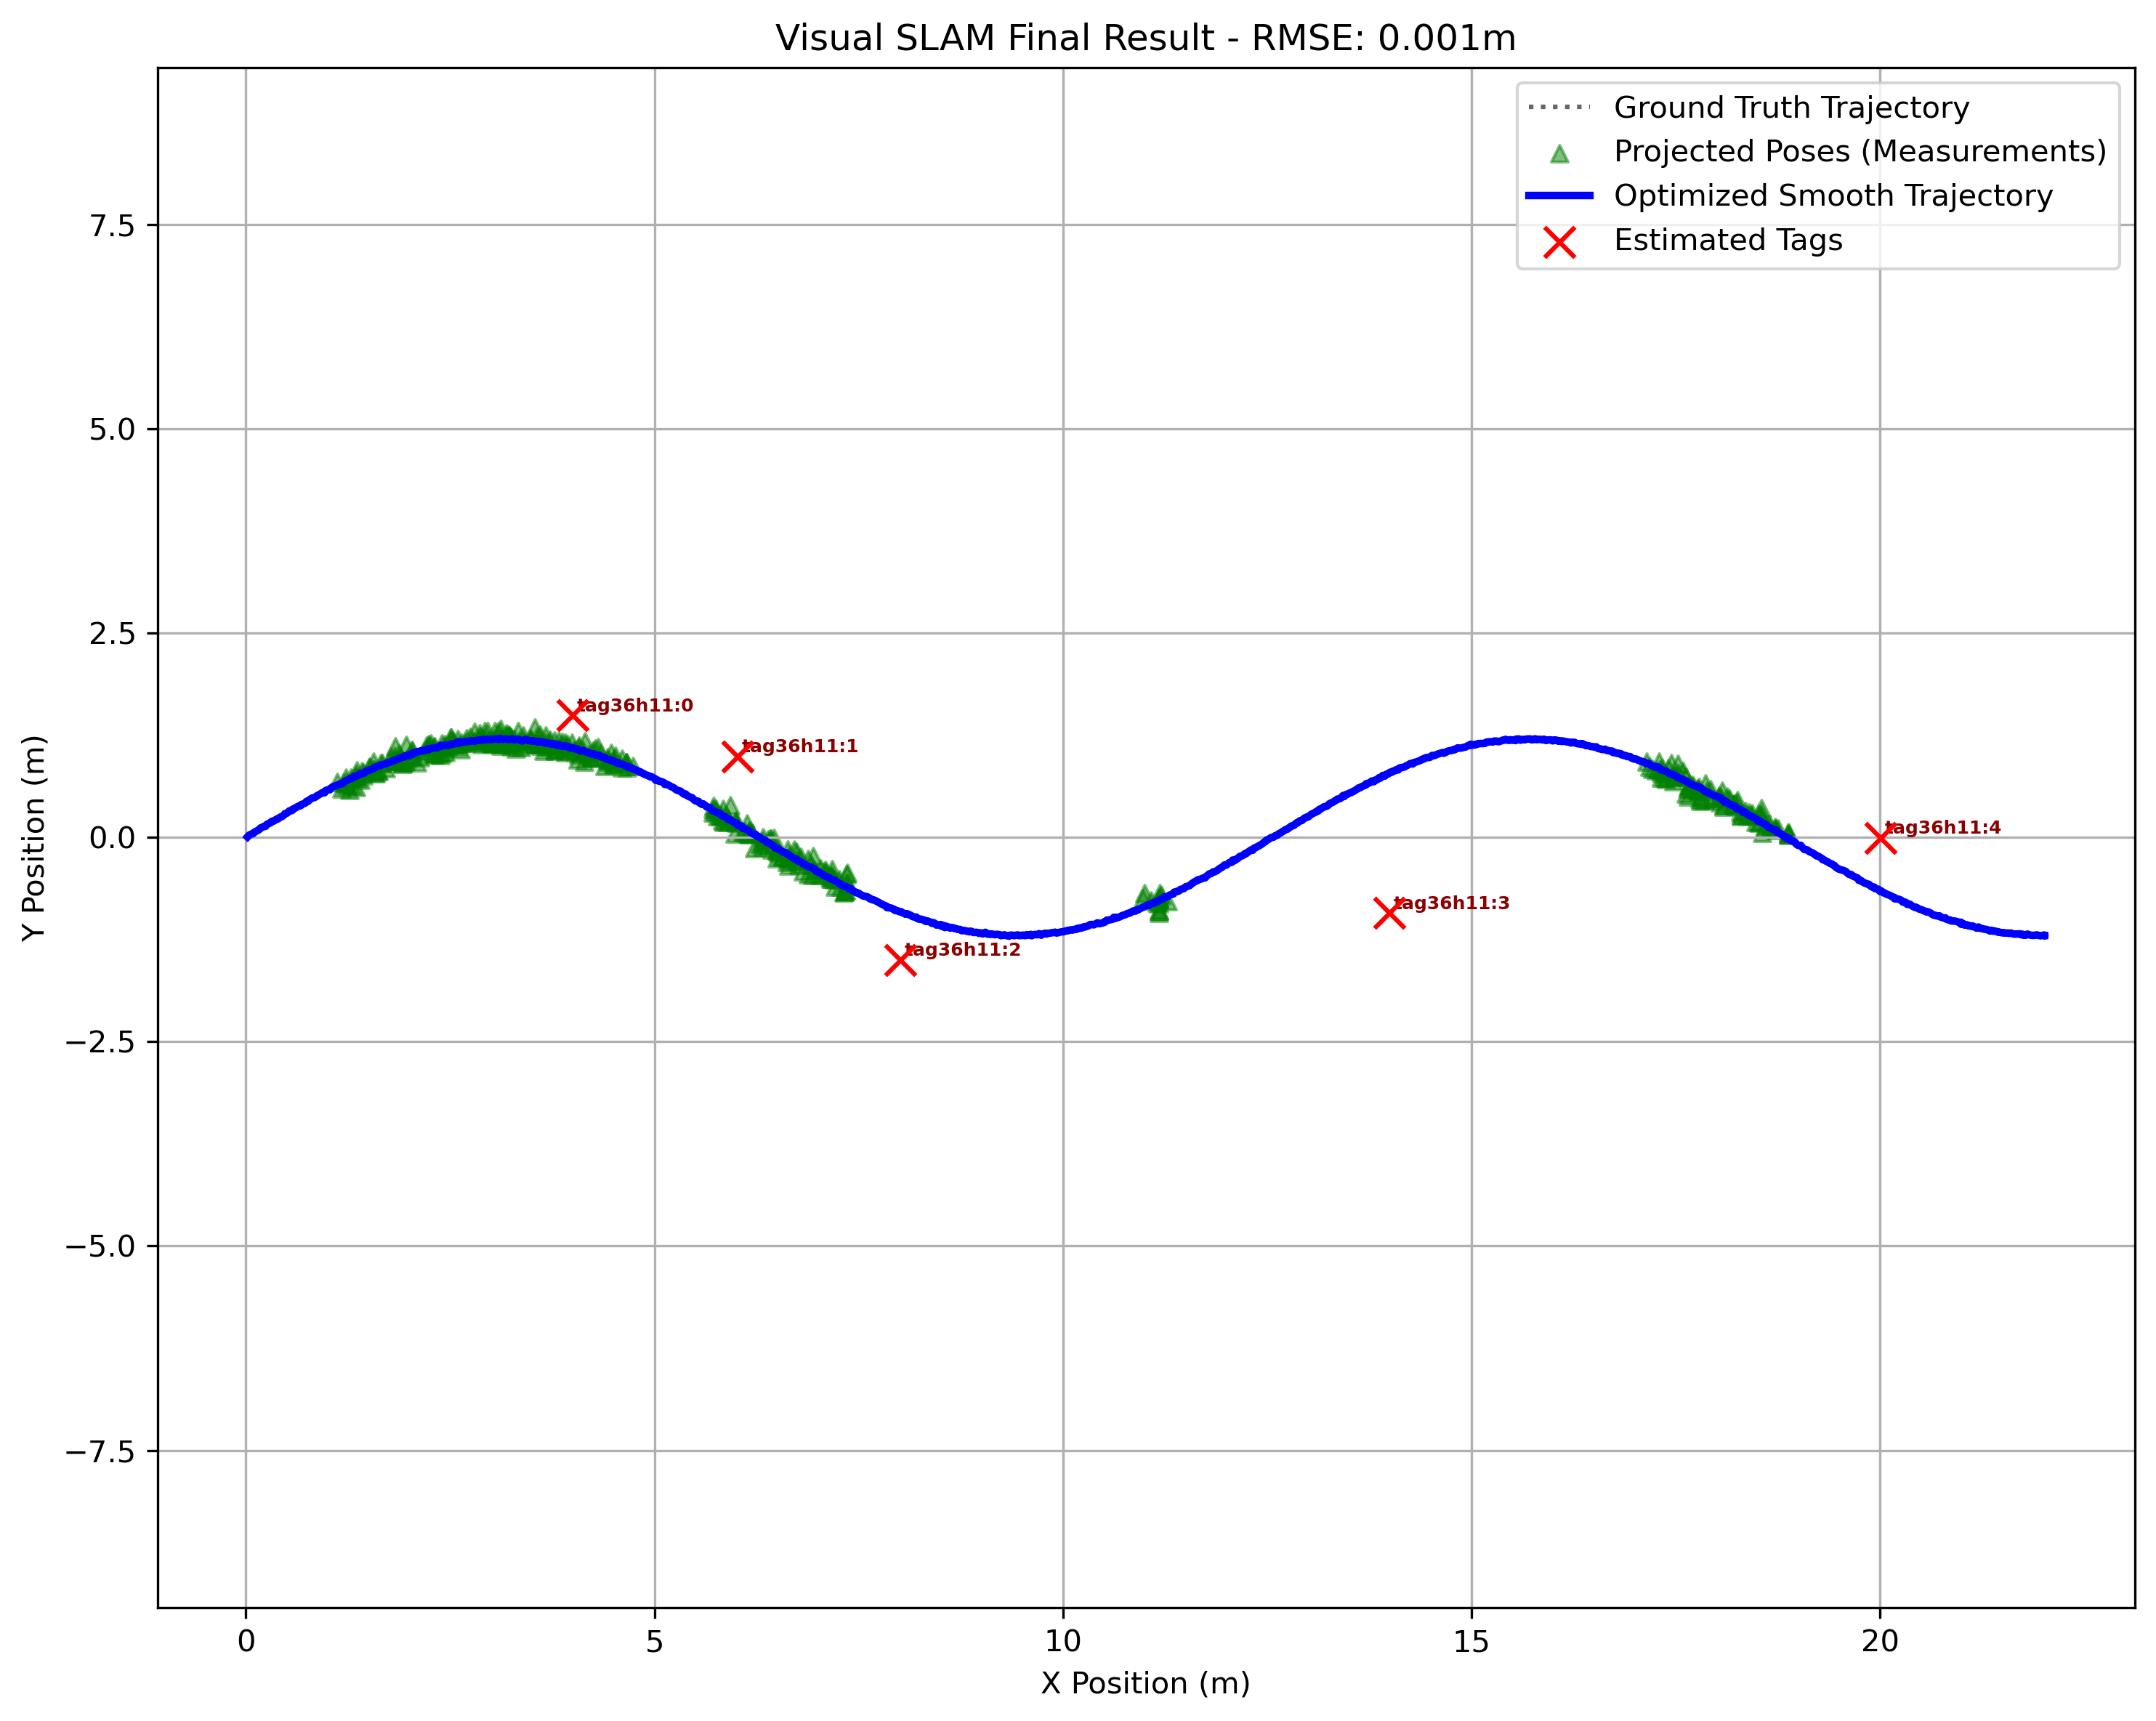
\includegraphics[width=\textwidth]{assets/slam_final__noise_graph.png}
            \vspace{0.2cm}
            {\small\textit{Fig. 7.1 — Simulated Dataset with Gaussian Noise}}
        \end{column}
        
        % COLUNA DIREITA: Caminho Otimizado/Recuperado
        
    \end{columns}
\end{frame}


\begin{frame}{Quantitative Analysis Sinusoidal Trajectory}
    \centering
    \footnotesize % Usa fonte um pouco menor para caber na coluna

    \begin{columns}[T] % Alinha o topo das colunas

        % ===================================
        % COLUNA 1: DADOS OTIMIZADOS SEM RUÍDO (Ideal - s_curve_otmires.png)
        % ===================================
        \begin{column}{0.48\textwidth}
            \centering
            \textbf{Case 1: Optimization without NOISE (Ideal)}
            \vspace{0.1cm}

            % Título principal dos resultados
            \begin{tabular}{lr}
                \toprule
                \textbf{Metric} & \textbf{Value} \\
                \midrule
                \textbf{Trajectory RMSE} & $\mathbf{0.0000 \text{ m}}$ \\ % Destacando o RMSE ideal
                Avg. Tag Position Error & $0.0164 \text{ m}$ \\
                \bottomrule
            \end{tabular}

            \vspace{0.3cm}
            
            % Tabela de Erro de Posição das AprilTags
            \textbf{Tag Estimation Error (Ideal)}
            \begin{tabular}{lccc}
                \toprule
                \textbf{Tag Name} & $\mathbf{X}$ \textbf{Error} & $\mathbf{Y}$ \textbf{Error} & $\mathbf{Z}$ \textbf{Error} \\
                \midrule
                tag36h11:0 & $0.00$ & $0.00$ & $0.00$ \\
                tag36h11:1 & $0.00$ & $0.00$ & $0.00$ \\
                tag36h11:2 & $0.01$ & $-0.01$ & $0.00$ \\
                tag36h11:3 & $0.03$ & $0.00$ & $0.00$ \\
                tag36h11:4 & $0.02$ & $-0.02$ & $0.00$ \\
                \bottomrule
            \end{tabular}
        \end{column}

        % LINHA VERTICAL (Opcional, para separar visualmente)
        \vrule width 0.1pt

        % ===================================
        % COLUNA 2: DADOS OTIMIZADOS COM RUÍDO (s_curve_noisy_otmires.png)
        % ===================================
        \begin{column}{0.48\textwidth}
            \centering
            \textbf{Case 2: Optimization with NOISE (6 cm)}
            \vspace{0.1cm}
            
            % Título principal dos resultados
            \begin{tabular}{lr}
                \toprule
                \textbf{Metric} & \textbf{Value} \\
                \midrule
                \textbf{Trajectory RMSE} & $\mathbf{0.0007 \text{ m}}$ \\ % Destacando o RMSE com ruído
                Avg. Tag Position Error & $0.0239 \text{ m}$ \\
                \bottomrule
            \end{tabular}

            \vspace{0.3cm}
            
            % Tabela de Erro de Posição das AprilTags
            \textbf{Tag Estimation Error}
            \begin{tabular}{lccc}
                \toprule
                \textbf{Tag Name} & $\mathbf{X}$ \textbf{Error} & $\mathbf{Y}$ \textbf{Error} & $\mathbf{Z}$ \textbf{Error} \\
                \midrule
                tag36h11:0 & $0.00$ & $0.01$ & $0.01$ \\
                tag36h11:1 & $0.01$ & $0.00$ & $0.00$ \\
                tag36h11:2 & $0.00$ & $-0.04$ & $0.01$ \\
                tag36h11:3 & $-0.01$ & $0.07$ & $0.00$ \\
                tag36h11:4 & $0.00$ & $-0.01$ & $0.00$ \\
                \bottomrule
            \end{tabular}
            
        \end{column}

    \end{columns}
    
    % LEGENDA FINAL
    \begin{center}
        \textit{Tables — Comparison of Optimization Results with and without noise.}
    \end{center}
\end{frame}



\begin{frame}{Recovery the Optimal Path Sinusoidal Trajectory}
    \centering
    
    % Título da seção (acima das colunas)
    \textbf{The scenario with 23 tags}
    \vspace{0.5cm}
    
    \begin{columns}
        
        % COLUNA 1 (ESQUERDA): Trajetória Recuperada (Recovery)
        \begin{column}{0.5\textwidth}
            \centering
            % Sua imagem de recuperação
            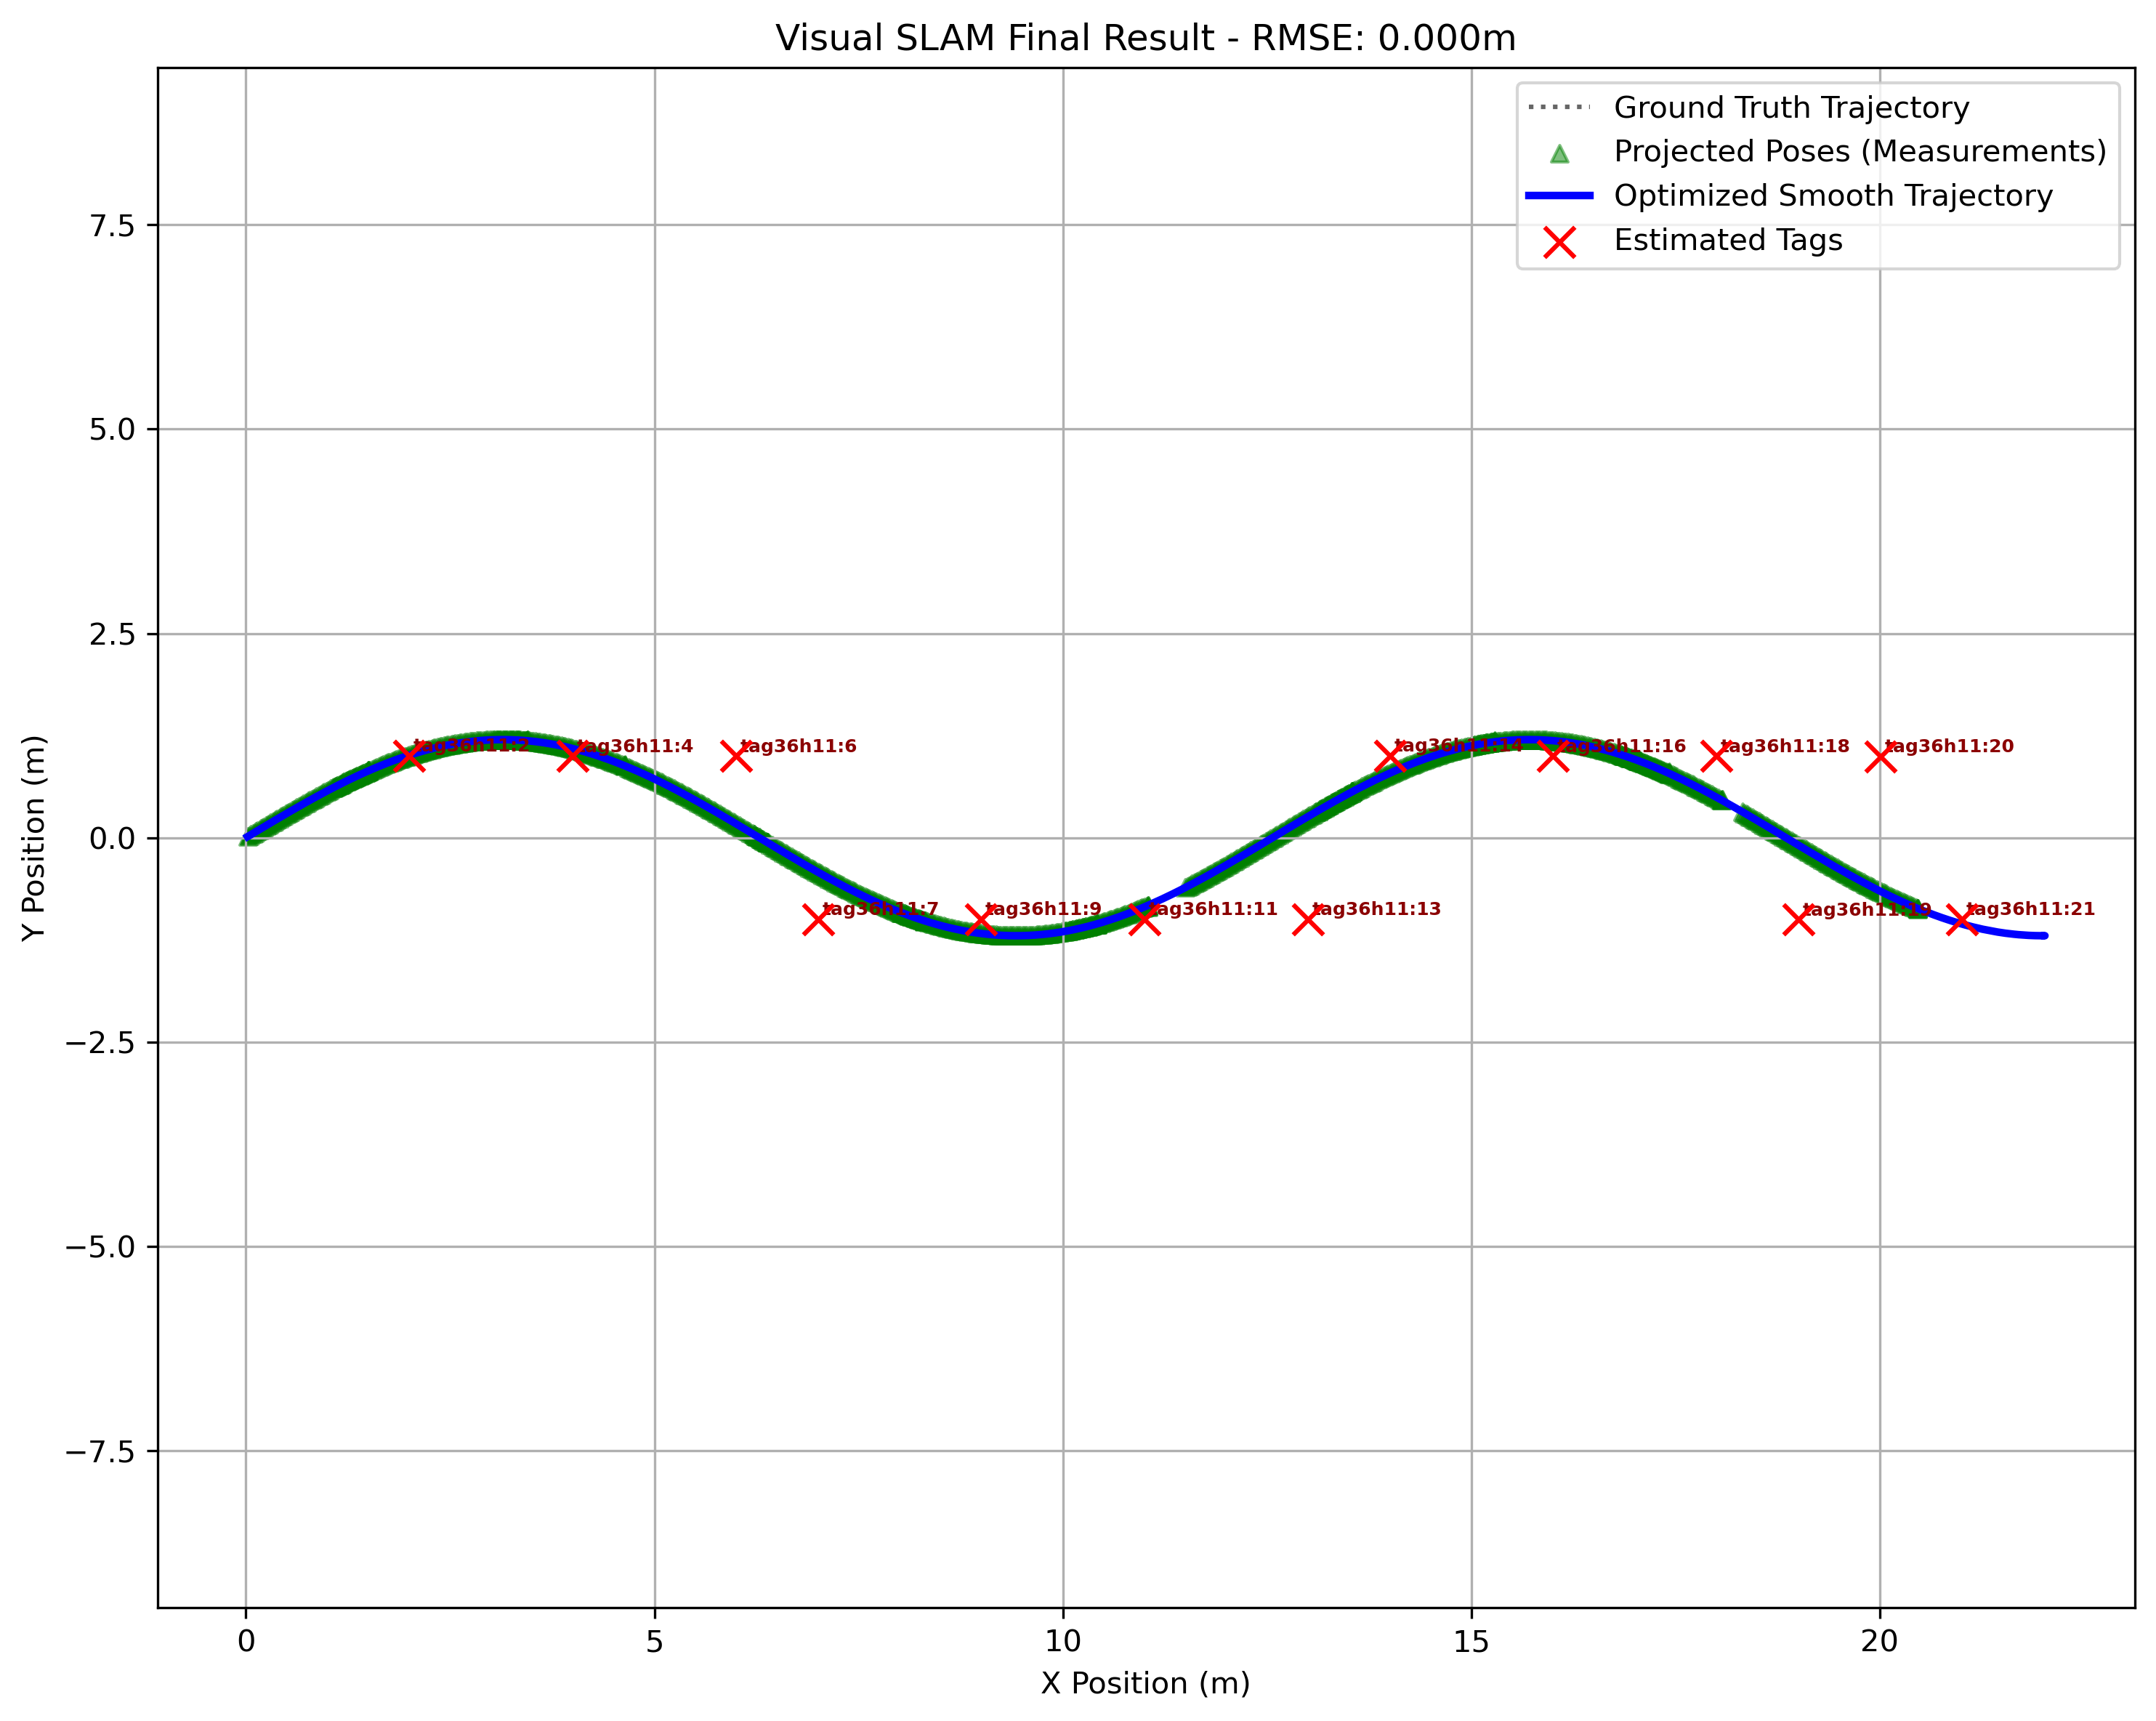
\includegraphics[width=\textwidth]{assets/s_20tags_final_graph.png}
            \vspace{0.2cm}
            {\small\textit{Fig. 8.1 — Trajectory Recovery via Optimization}} % Renomeei para 8.1 para manter a ordem lógica na tela
        \end{column}

        % COLUNA 2 (DIREITA): Dataset Ruidoso (Noisy Data)
        \begin{column}{0.5\textwidth}
            \centering
            % Imagem do dataset ruidoso da Phase 2
            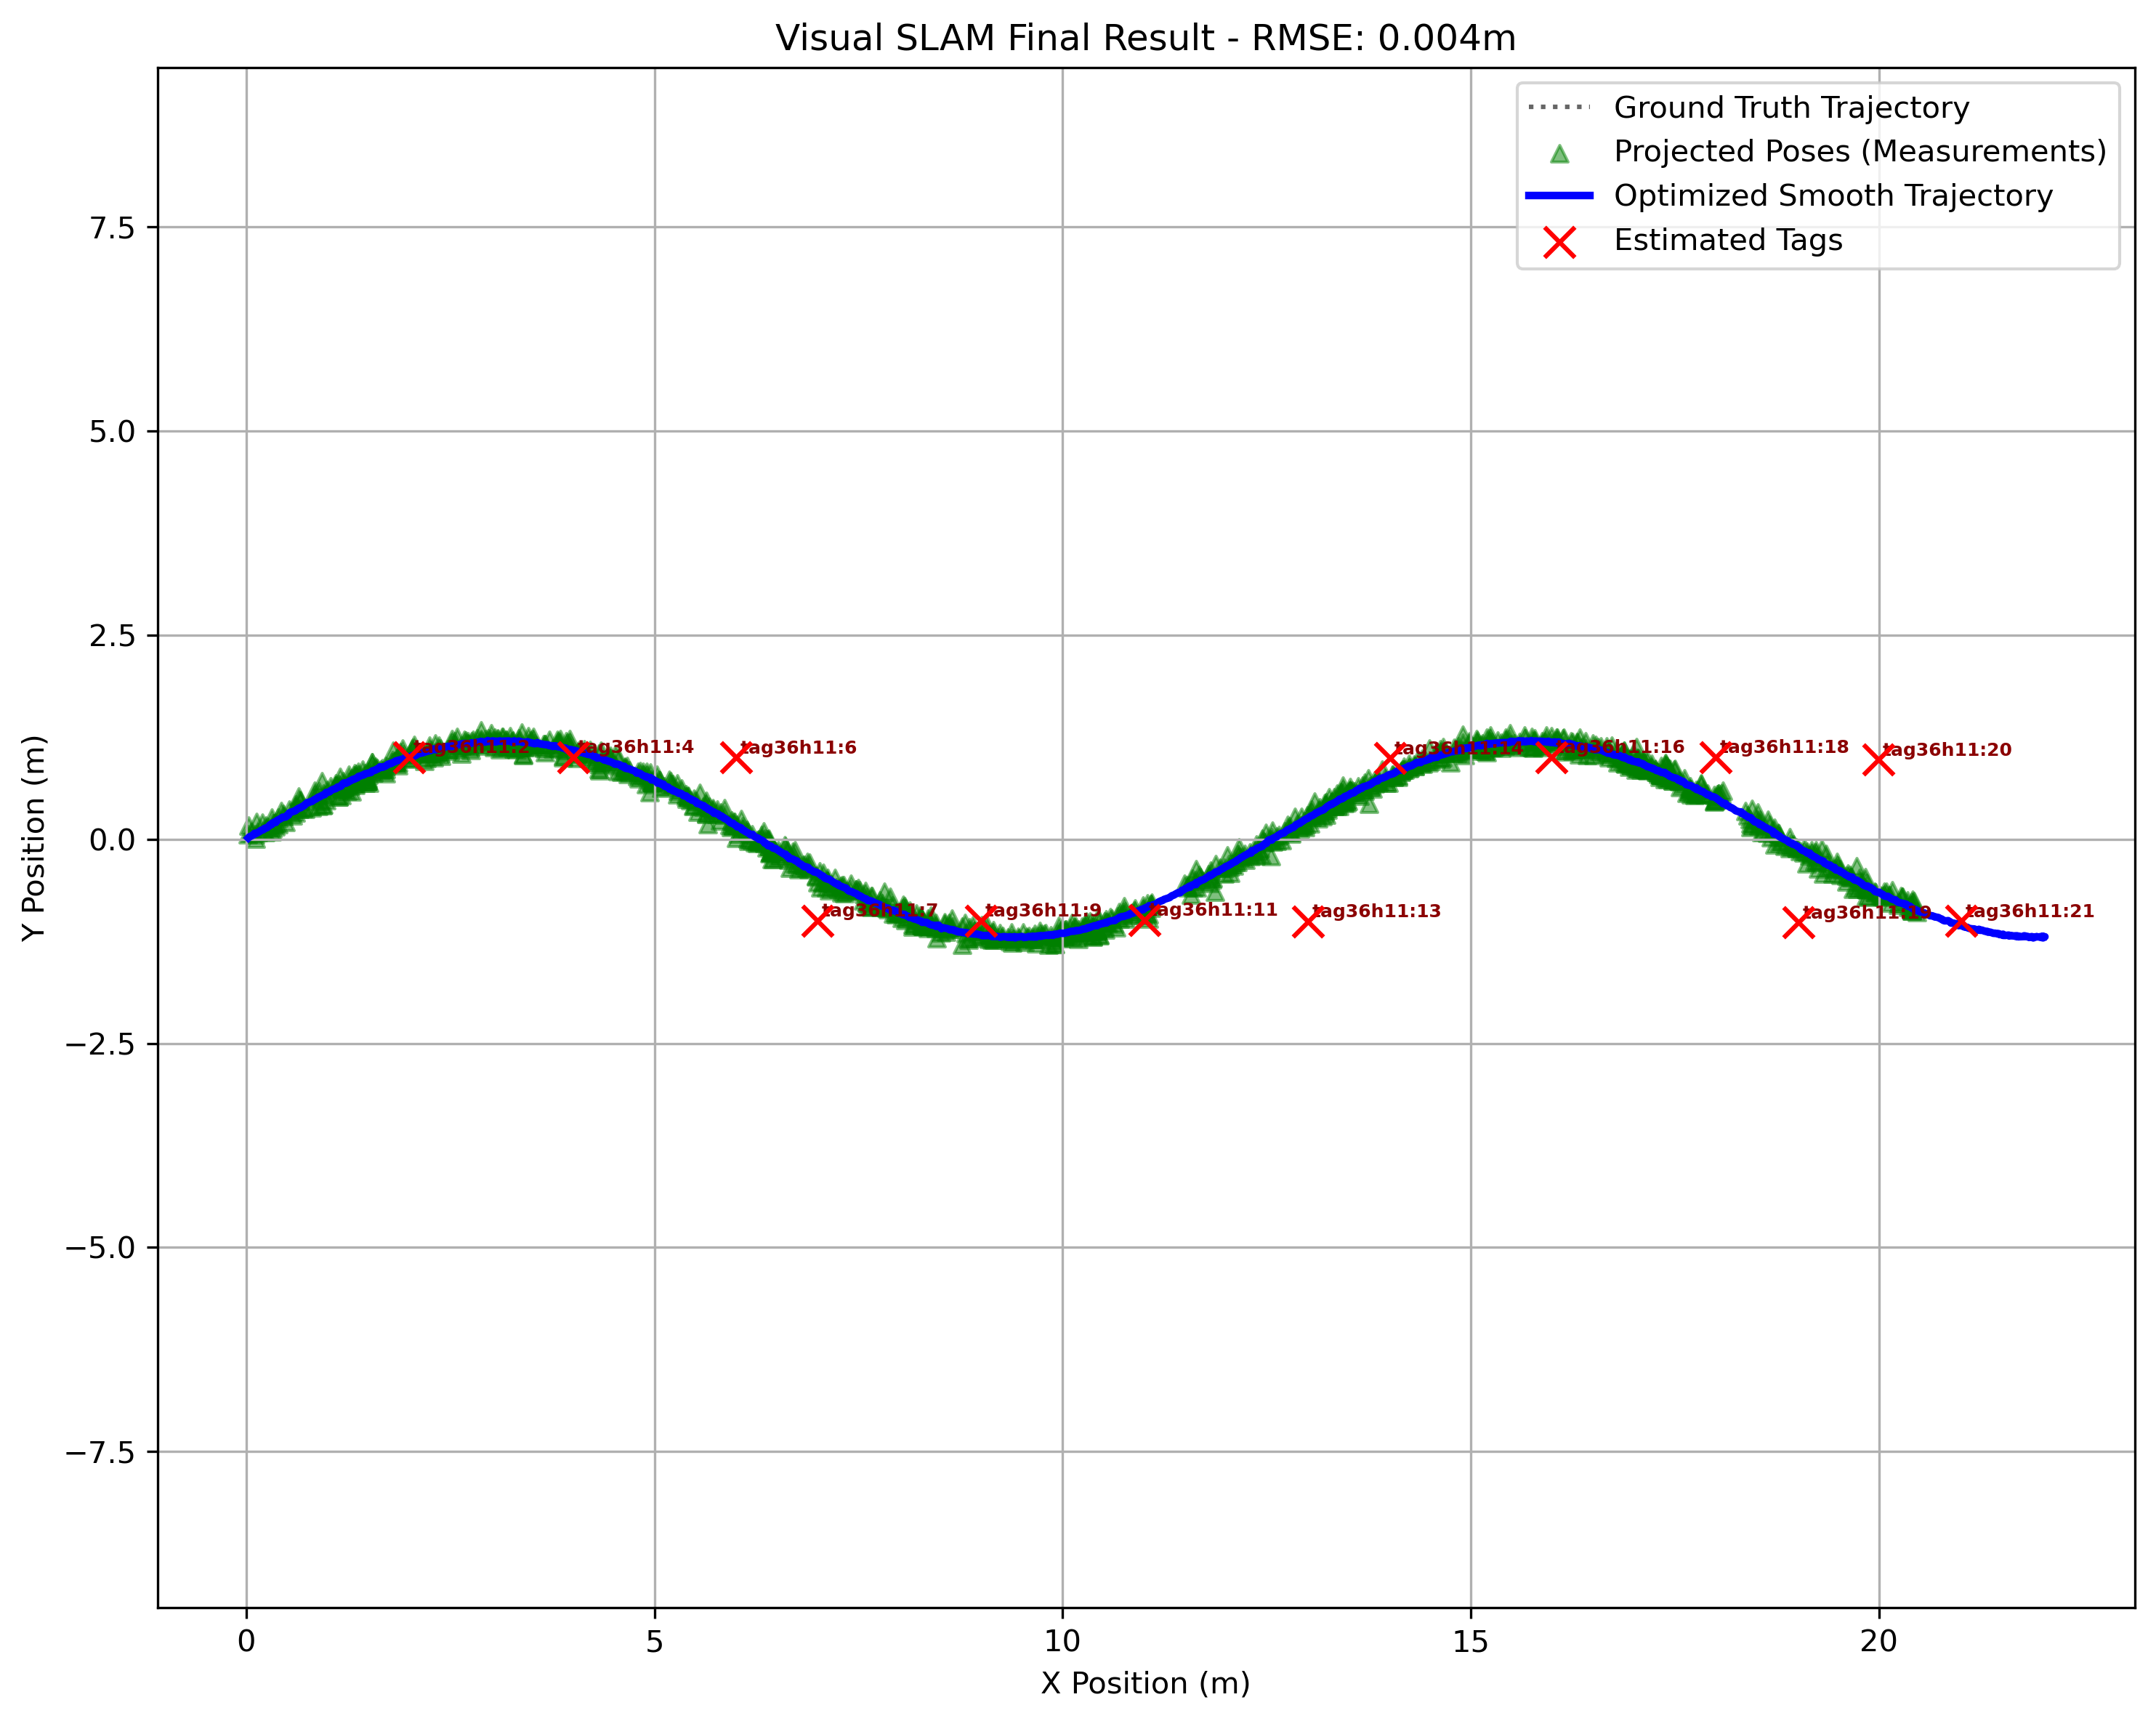
\includegraphics[width=\textwidth]{assets/s_20tags_noise_final_graph.png}
            \vspace{0.2cm}
            {\small\textit{Fig. 8.2 — Simulated Dataset with Gaussian Noise}} % Renomeei para 8.2
        \end{column}
        
    \end{columns}
\end{frame}

\begin{frame}{Quantitative Analysis Sinusoidal Trajectory }
    \centering
    \footnotesize % Usa fonte um pouco menor para caber na coluna

    \centering
    
    % Título da seção (acima das colunas)
    \textbf{The scenario with 23 tags}
    \vspace{0.5cm}

    \begin{columns}[T] % Alinha o topo das colunas

        % ===================================
        % COLUNA 1: DADOS OTIMIZADOS SEM RUÍDO (Ideal - s_20tags_curve_otmires.png)
        % ===================================
        \begin{column}{0.48\textwidth}
            \centering
            \textbf{Case 1: Optimization without NOISE} 
            \vspace{0.1cm}

            % Tabela de Métricas (Mantida)
            \begin{tabular}{lr}
                \toprule
                \textbf{Metric} & \textbf{Value} \\
                \midrule
                \textbf{Trajectory RMSE} & $\mathbf{0.0002 \text{ m}}$ \\ 
                Avg. Tag Position Error & $0.0019 \text{ m}$ \\
                \bottomrule
            \end{tabular}

            \vspace{0.3cm}
            
            % Tabela de Erro de Posição das AprilTags (AMOSTRA)
            \textbf{Tag Estimation Error (Sample)}
            \begin{tabular}{lccc}
                \toprule
                \textbf{Tag Name} & $\mathbf{X}$ \textbf{Error} & $\mathbf{Y}$ \textbf{Error} & $\mathbf{Z}$ \textbf{Error} \\
                \midrule
                tag36h11:2 & $0.00$ & $0.00$ & $0.00$ \\
                tag36h11:7 & $0.00$ & $0.00$ & $0.00$ \\
                tag36h11:13 & $0.00$ & $0.00$ & $0.00$ \\
                tag36h11:18 & $0.00$ & $0.00$ & $0.00$ \\
                tag36h11:21 & $0.00$ & $0.00$ & $0.00$ \\
                \bottomrule
            \end{tabular}
        \end{column}

        % LINHA VERTICAL
        \vrule width 0.1pt

        % ===================================
        % COLUNA 2: DADOS OTIMIZADOS COM RUÍDO (s_20tags_curve_noisy_otmires.png)
        % ===================================
        \begin{column}{0.48\textwidth}
            \centering
            \textbf{Case 2: Optimization with NOISE (6 cm)} 
            \vspace{0.1cm}
            
            % Tabela de Métricas (Mantida)
            \begin{tabular}{lr}
                \toprule
                \textbf{Metric} & \textbf{Value} \\
                \midrule
                \textbf{Trajectory RMSE} & $\mathbf{0.0037 \text{ m}}$ \\ 
                Avg. Tag Position Error & $0.0134 \text{ m}$ \\
                \bottomrule
            \end{tabular}

            \vspace{0.3cm}
            
            % Tabela de Erro de Posição das AprilTags (AMOSTRA)
            \textbf{Tag Estimation Error (Sample)}
            \begin{tabular}{lccc}
                \toprule
                \textbf{Tag Name} & $\mathbf{X}$ \textbf{Error} & $\mathbf{Y}$ \textbf{Error} & $\mathbf{Z}$ \textbf{Error} \\
                \midrule
                tag36h11:2 & $0.01$ & $0.01$ & $0.00$ \\
                tag36h11:7 & $0.00$ & $0.00$ & $0.00$ \\
                tag36h11:13 & $0.01$ & $0.01$ & $0.00$ \\
                tag36h11:18 & $0.00$ & $0.00$ & $0.01$ \\
                tag36h11:21 & $0.01$ & $0.00$ & $0.02$ \\
                \bottomrule
            \end{tabular}
            
        \end{column}

    \end{columns}
    
    % LEGENDA FINAL
    \begin{center}
        \textit{Tables — Comparison of Optimization Results with and without noise (Sample of 5 Tags).}
    \end{center}
\end{frame}

\begin{frame}{Recovery the Optimal Path: Straight Trajectory}
    \centering
    
    \begin{columns}
        
        % COLUMN 1 (LEFT): Trajectory Recovery (Optimized)
        \begin{column}{0.5\textwidth}
            \centering
            % Assuming image name for the optimized straight trajectory
            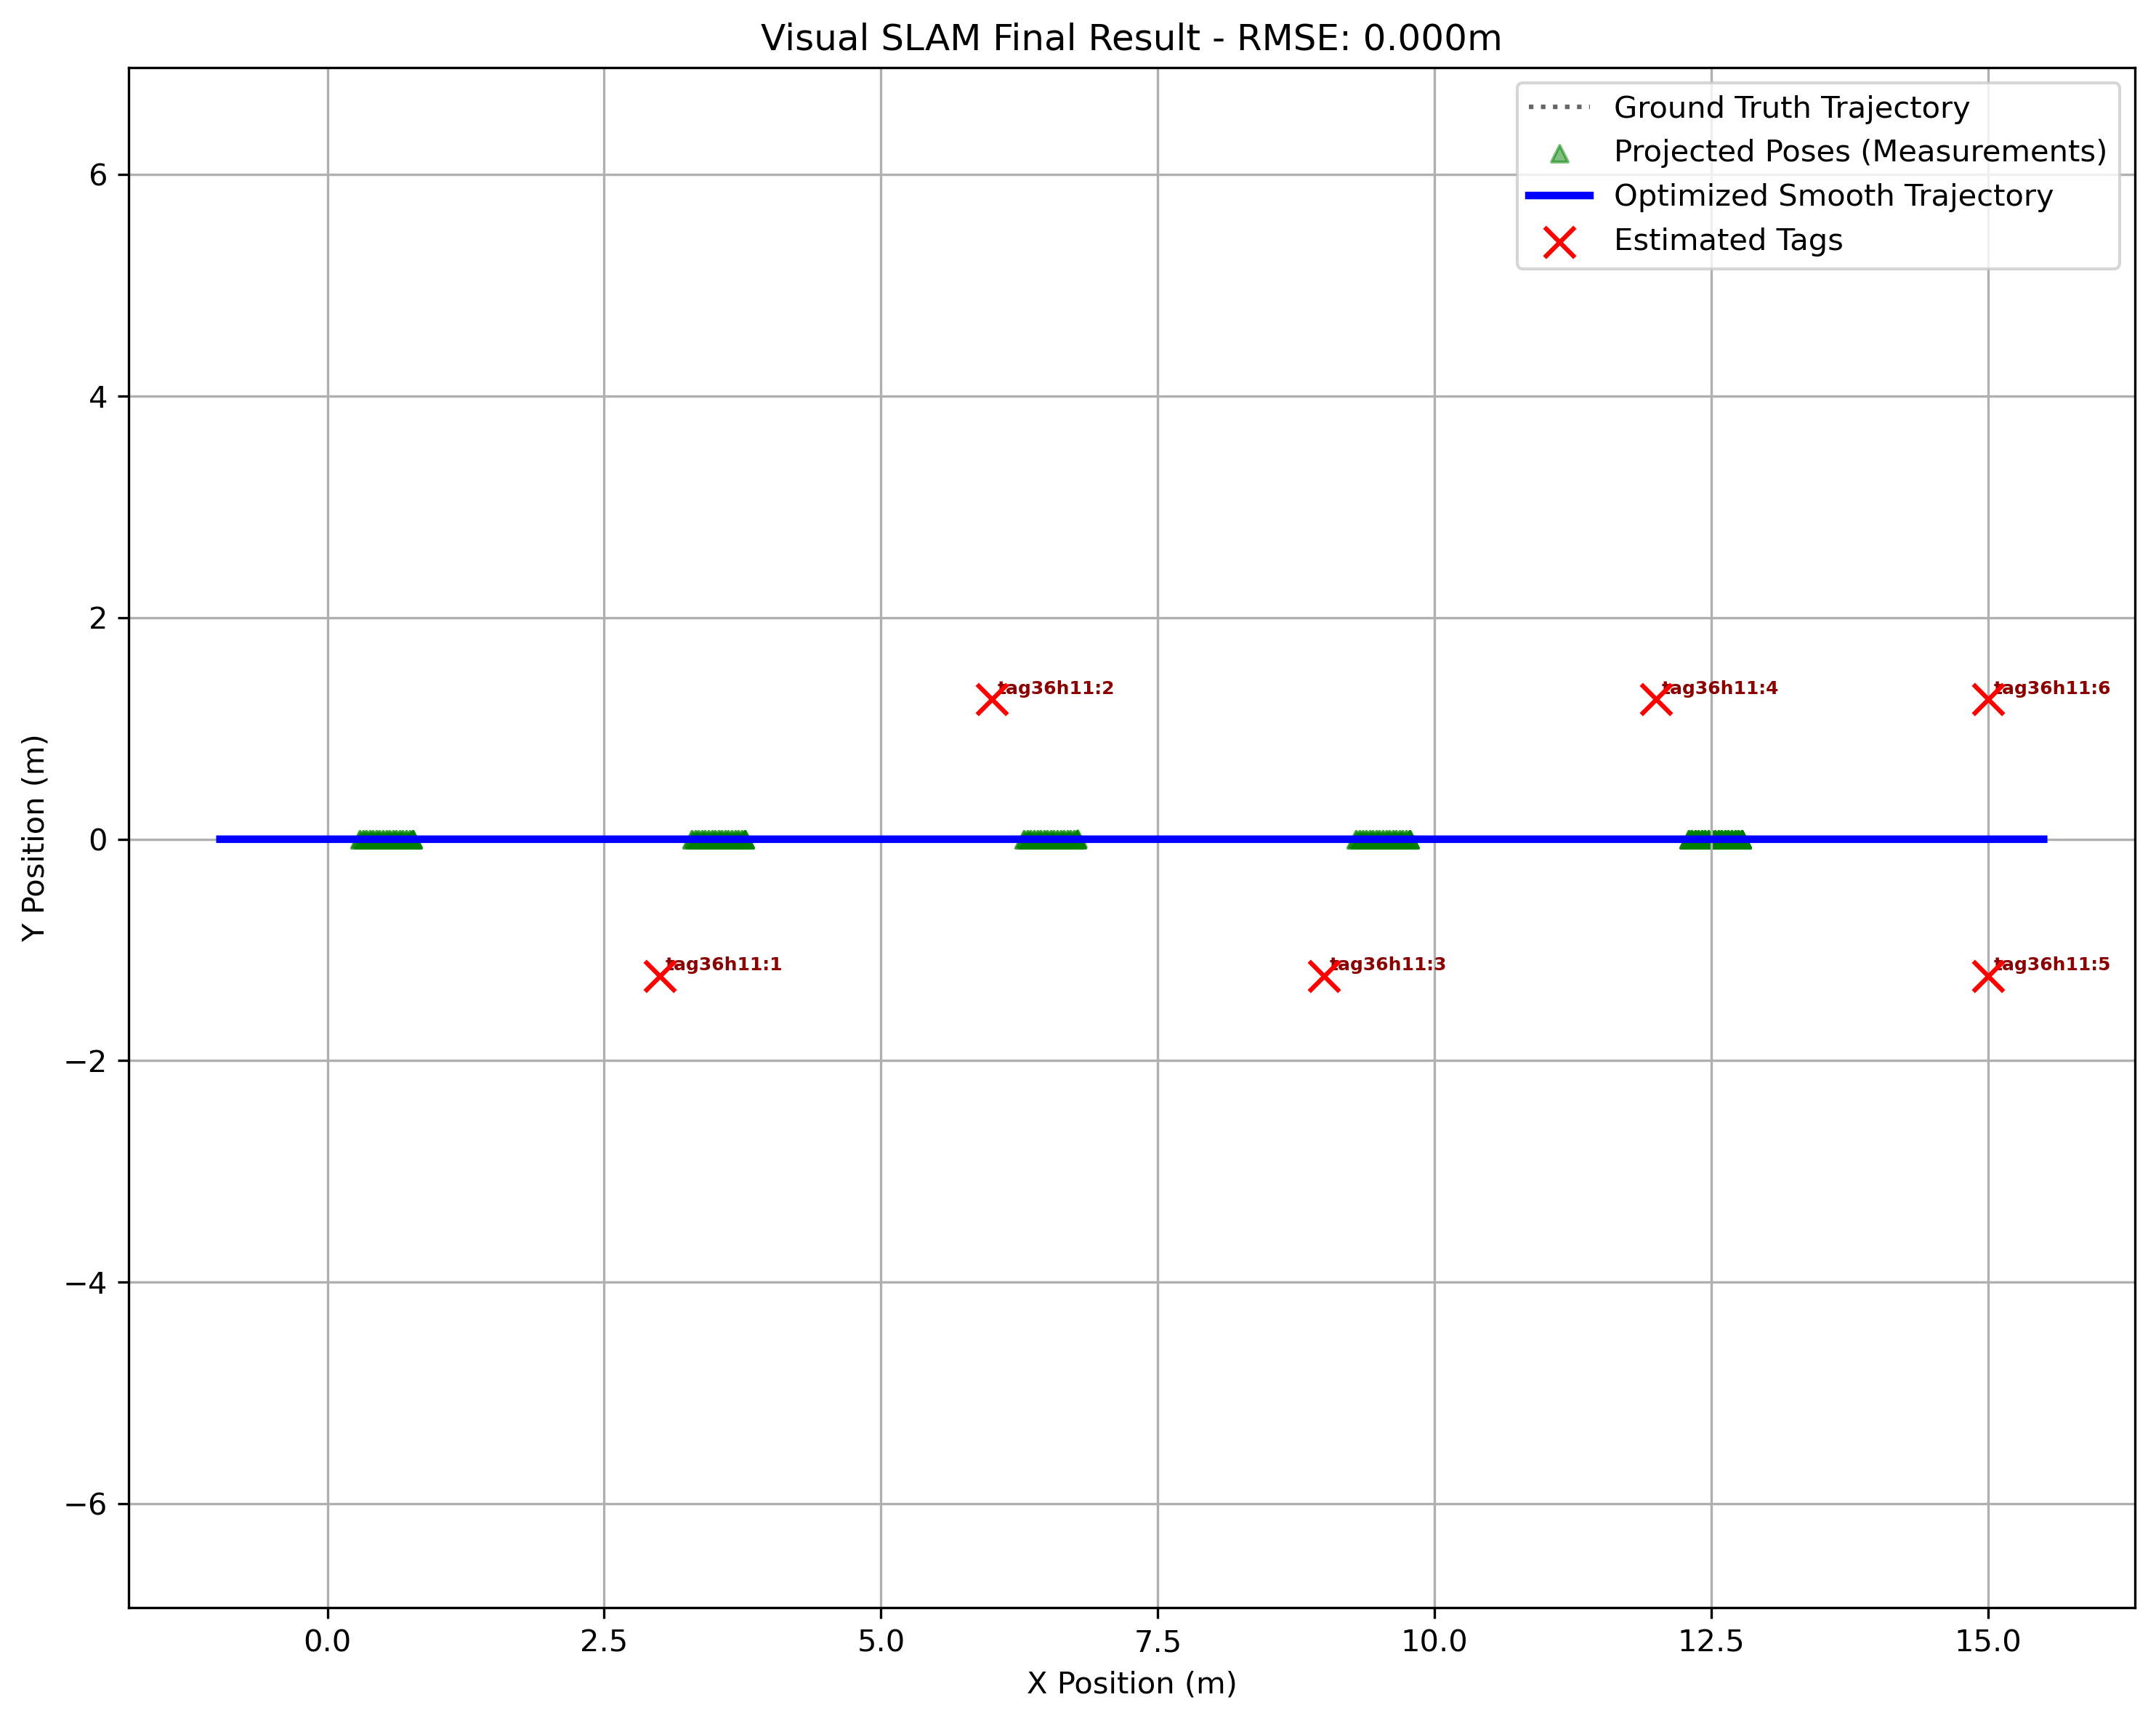
\includegraphics[width=\textwidth]{assets/straight_final_graph.png}
            \vspace{0.2cm}
            {\small\textit{Fig. 8.1 — Trajectory Recovery via Optimization}} 
        \end{column}

        % COLUMN 2 (RIGHT): Noisy Dataset
        \begin{column}{0.5\textwidth}
            \centering
            % Assuming image name for the noisy straight trajectory dataset
            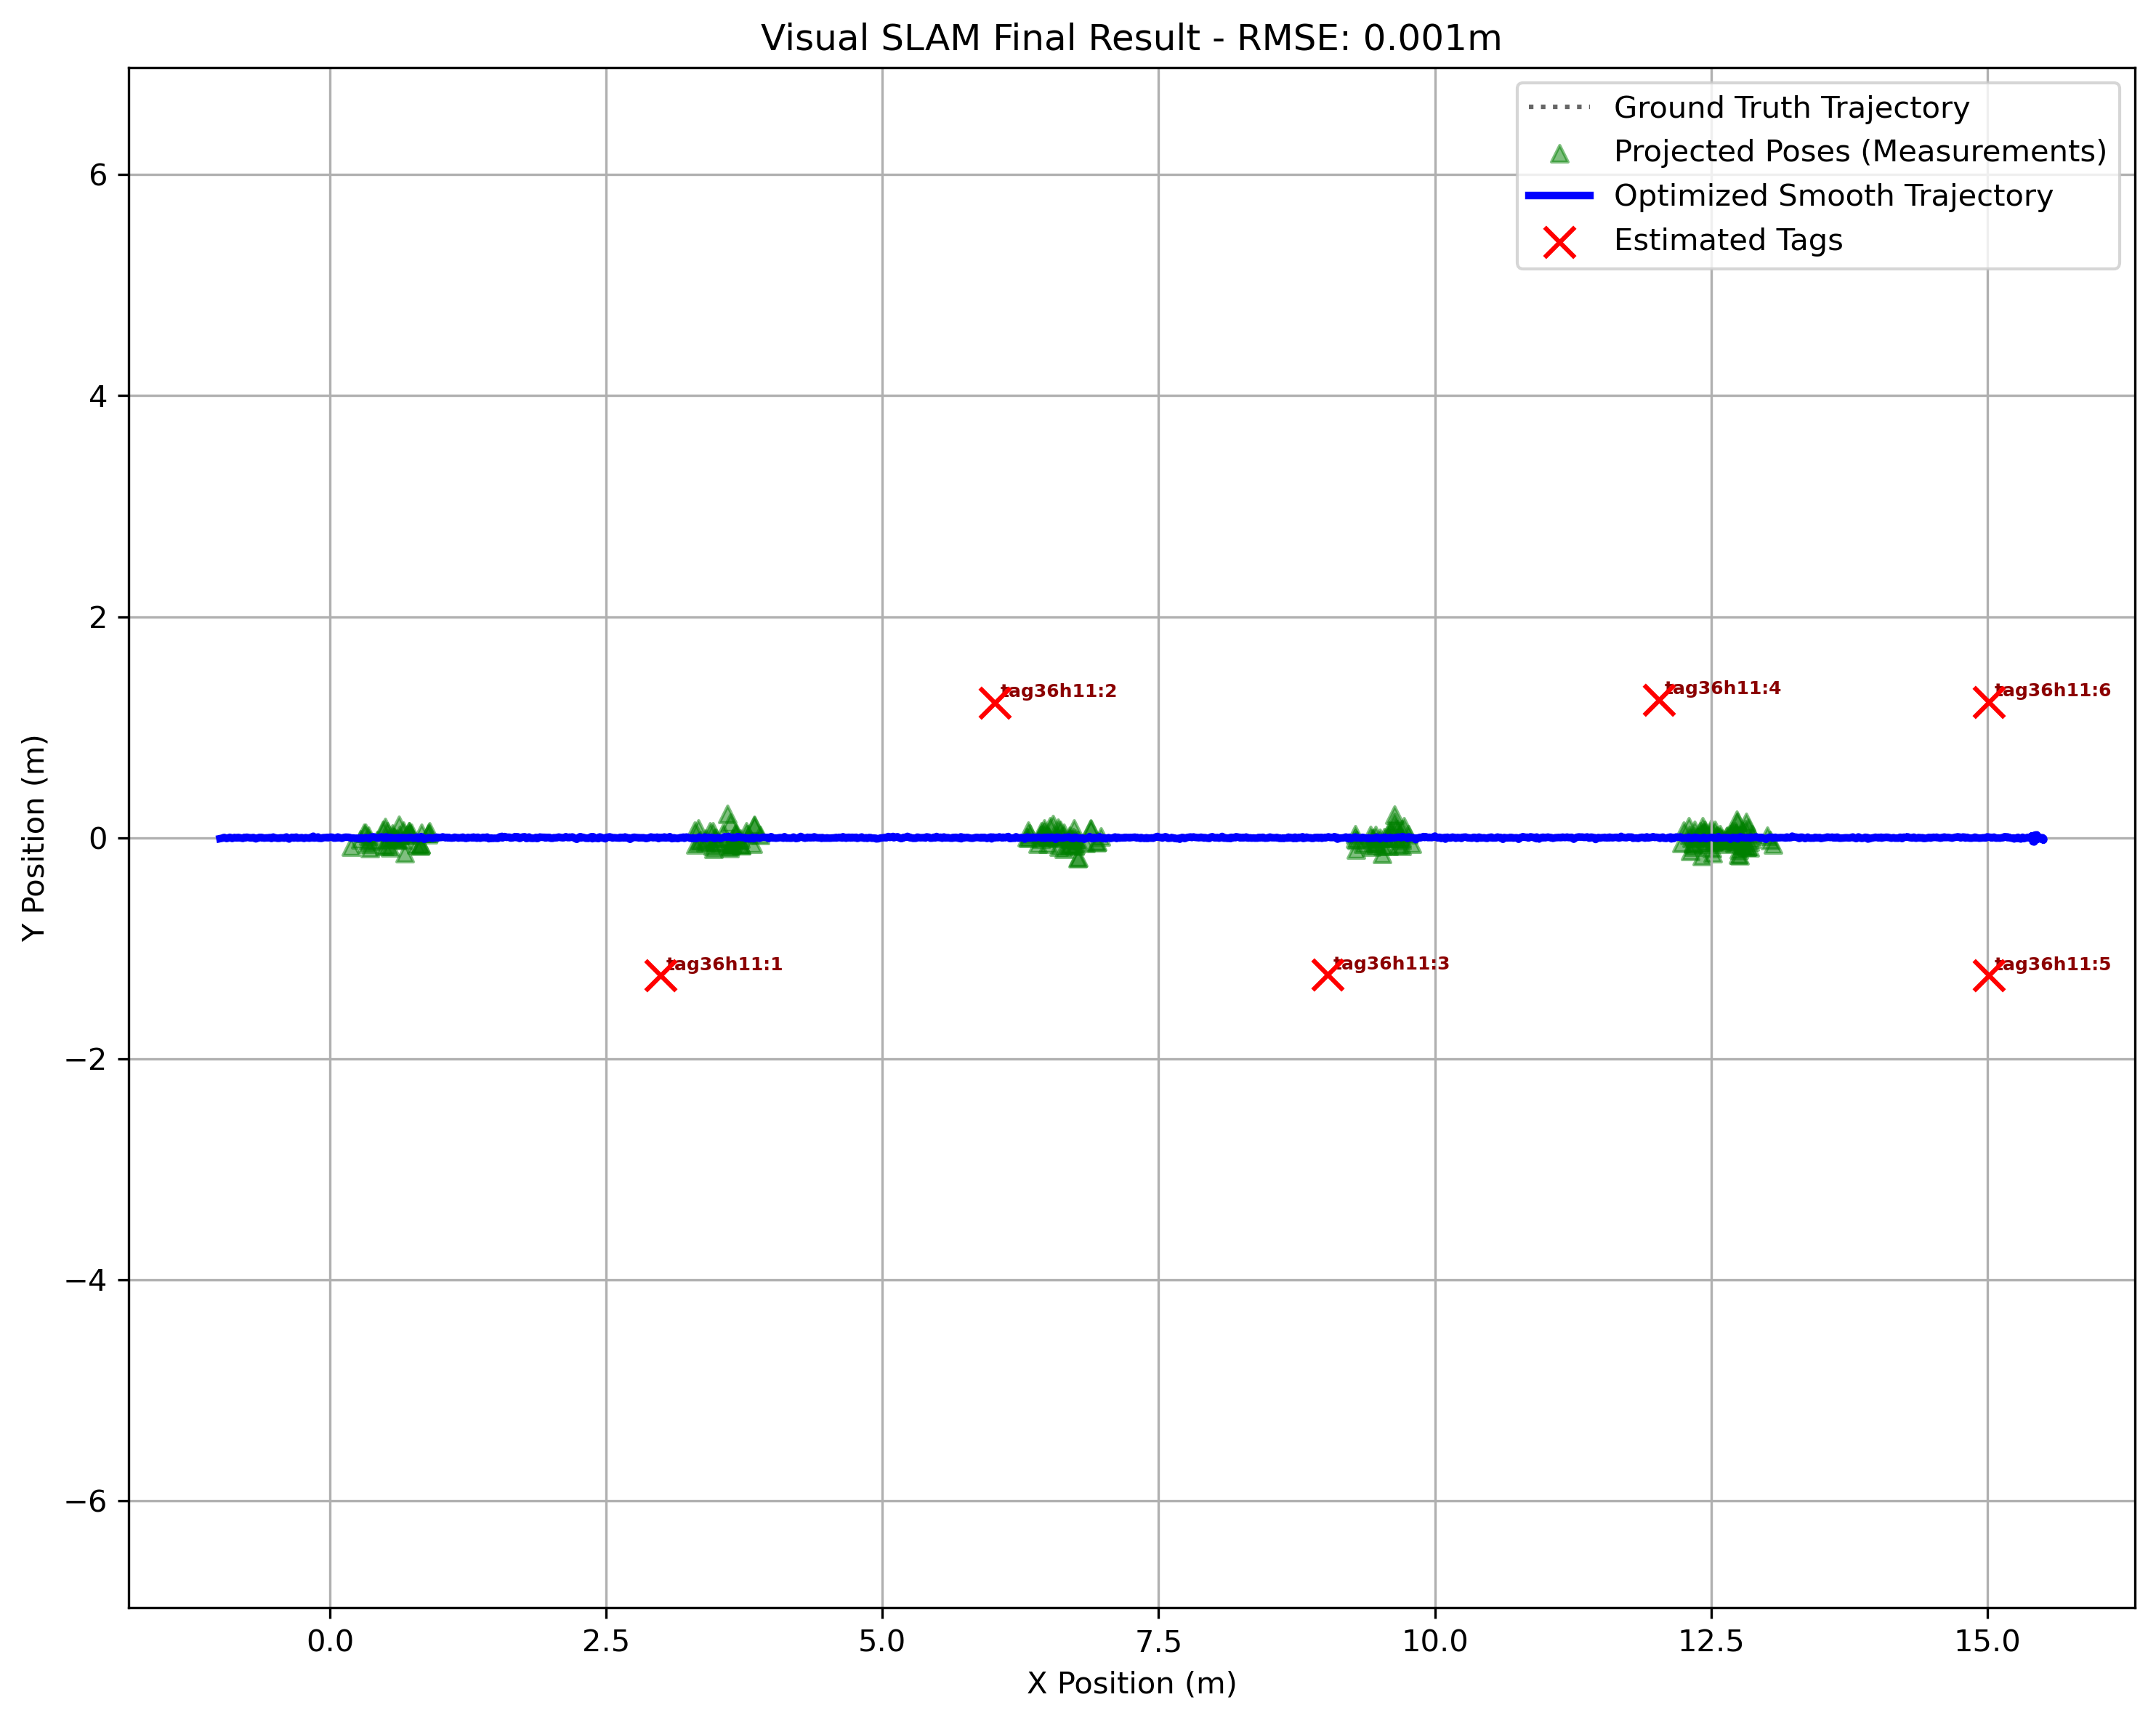
\includegraphics[width=\textwidth]{assets/straight_noisy_final_graph.png}
            \vspace{0.2cm}
            {\small\textit{Fig. 8.2 — Simulated Dataset with Gaussian Noise}} 
        \end{column}
        
    \end{columns}
\end{frame}

\begin{comment}


\begin{frame}{Quantitative Analysis: Straight Trajectory}
    \centering
    \footnotesize % Use smaller font size to fit content

    \begin{columns}[T] % Align the top of the columns

        % ===================================
        % COLUMN 1: DATA WITHOUT NOISE (IDEAL)
        % ===================================
        \begin{column}{0.48\textwidth}
            \centering
            {\tiny (Data Source: straight\_otmires.png)}
            \vspace{0.1cm}
            
            \textbf{Case 1: Optimization without NOISE}
            \vspace{0.1cm}

            % Metrics Table
            \begin{tabular}{lr}
                \toprule
                \textbf{Metric} & \textbf{Value} \\
                \midrule
                \textbf{Trajectory RMSE} & $\mathbf{0.0017 \text{ m}}$ \\
                Avg. Tag Position Error & $\mathbf{0.0000 \text{ m}}$ \\
                \bottomrule
            \end{tabular}

            \vspace{0.3cm}
            
            % Tag Estimation Error Table
            \textbf{Tag Estimation Error (Ideal)}
            \begin{tabular}{lc}
                \toprule
                \textbf{Tag Name} & \textbf{Error (m)} \\
                \midrule
                tag36h11:1 & $0.0000$ \\
                tag36h11:2 & $0.0000$ \\
                tag36h11:3 & $0.0000$ \\
                tag36h11:4 & $0.0000$ \\
                tag36h11:5 & $0.0000$ \\
                tag36h11:6 & $0.0000$ \\
                \bottomrule
            \end{tabular}
        \end{column}

        % VERTICAL LINE
        \vrule width 0.1pt

        % ===================================
        % COLUMN 2: DATA WITH NOISE
        % ===================================
        \begin{column}{0.48\textwidth}
            \centering
            {\tiny (Data Source: straight\_noisy\_otmires.png)}
            \vspace{0.1cm}
            
            \textbf{Case 2: Optimization with NOISE}
            \vspace{0.1cm}
            
            % Metrics Table
            \begin{tabular}{lr}
                \toprule
                \textbf{Metric} & \textbf{Value} \\
                \midrule
                \textbf{Trajectory RMSE} & $\mathbf{0.0007 \text{ m}}$ \\
                Avg. Tag Position Error & $\mathbf{0.0248 \text{ m}}$ \\
                \bottomrule
            \end{tabular}

            \vspace{0.3cm}
            
            % Tag Estimation Error Table
            \textbf{Tag Estimation Error}
            \begin{tabular}{lc}
                \toprule
                \textbf{Tag Name} & \textbf{Error (m)} \\
                \midrule
                tag36h11:1 & $0.0115$ \\
                tag36h11:2 & $0.0337$ \\
                tag36h11:3 & $0.0363$ \\
                tag36h11:4 & $0.0288$ \\
                tag36h11:5 & $0.0139$ \\
                tag36h11:6 & $0.0245$ \\
                \bottomrule
            \end{tabular}
            
        \end{column}

    \end{columns}
    
    % FINAL CAPTION
    \begin{center}
        \textit{Comparison: Ideal Case vs. Noisy Case (Results from Python Optimization)}
    \end{center}
\end{frame}


% ==================/// PHASE 4 ///==================
\begin{frame}{Phase 4: Robot implementation}
    \begin{columns}[T] % [T] Alinha o conteúdo pelo topo
        
        % --- Coluna da Esquerda (Texto) ---
        \begin{column}{0.6\textwidth}
            \textbf{Goal: Move from PC tests to the LIMOS robot}
            \vspace{0.5cm}
            \begin{itemize}
                \setlength\itemsep{1em} % Espaçamento entre itens
                
                \item<1-> \textbf{Onboard integration:}  
                Put the perception code on the robot (ROS~2).

                \item<3-> \textbf{Camera calibration:}  
                Calibrate the camera so distances look right.

                \item<5-> \textbf{First trajectory recording:}  
                Record one path using wheels plus AprilTag pose.
            \end{itemize}
        \end{column}
        
        % --- Coluna da Direita (Imagens) ---
        \begin{column}{0.38\textwidth}
            \centering
            % overlayarea reserva o espaço para evitar que o slide pule na troca
            \begin{overlayarea}{\textwidth}{0.6\textheight}
                \centering
                
                % IMAGEM 1: Aparece no slide 2 e SOME no final do slide 3
                \only<2>{
                    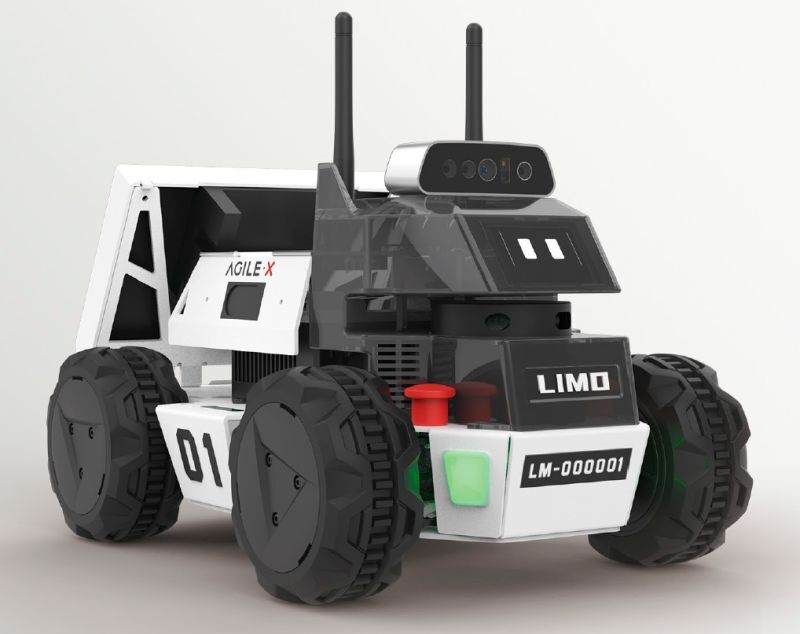
\includegraphics[width=\textwidth, keepaspectratio]{assets/limo.jpeg}
                    \vspace{0cm}
                    \\{\tiny\textit{Fig. 8 — LIMOS platform}}
                }sinusoidal
                
                % IMAGEM 2: Aparece no slide 4 e fica até o fim
                % (Coloquei o mesmo nome de arquivo, mas idealmente seria outra foto)
                \only<4->{
                    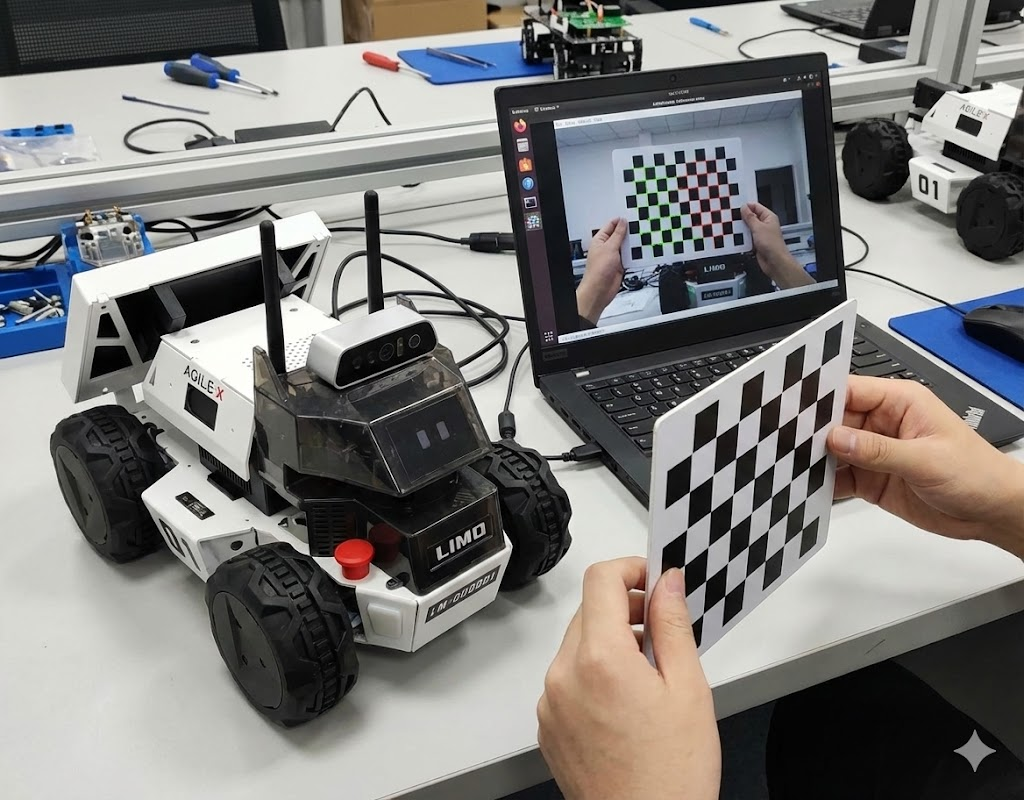
\includegraphics[trim={5cm 3cm 5cm 2cm}, clip, width=\textwidth]{assets/camera_calibration.jpg}
                    \vspace{0cm}
                    \\{\tiny\textit{Fig. 9 — Calibration}}
                }
            \end{overlayarea}
        \end{column}
        
    \end{columns}
\end{frame}

\end{comment}


\begin{frame}{Quantitative Analysis: Straight Trajectory}
    \centering
    \footnotesize % Use smaller font size to fit content

    \centering
    


    \begin{columns}[T] % Align the top of the columns

        % ===================================
        % COLUMN 1: DATA WITHOUT NOISE
        % ===================================
        \begin{column}{0.48\textwidth}
            \centering
            % Texto da fonte

            \vspace{0.1cm}
            
            \textbf{Case 1: Optimization without NOISE}
            \vspace{0.1cm}

            % Metrics Table
            \begin{tabular}{lr}
                \toprule
                \textbf{Metric} & \textbf{Value} \\
                \midrule
                \textbf{Trajectory RMSE} & $\mathbf{0.0017 \text{ m}}$ \\
                Avg. Tag Position Error & $0.0000 \text{ m}$ \\
                \bottomrule
            \end{tabular}

            \vspace{0.3cm}
            
            % Tag Estimation Error Table
            \textbf{Tag Estimation Error (Sample)}
            \begin{tabular}{lccc}
                \toprule
                \textbf{Tag Name} & $\mathbf{X}$ \textbf{Error} & $\mathbf{Y}$ \textbf{Error} & $\mathbf{Z}$ \textbf{Error} \\
                \midrule
                tag36h11:0 & $0.00$ & $0.00$ & $0.00$ \\
                tag36h11:1 & $0.00$ & $0.00$ & $0.00$ \\
                tag36h11:2 & $0.00$ & $0.00$ & $0.00$ \\
                tag36h11:3 & $0.00$ & $0.00$ & $0.00$ \\
                tag36h11:4 & $0.00$ & $0.00$ & $0.00$ \\
                \bottomrule
            \end{tabular}
        \end{column}

        % VERTICAL LINE
        \vrule width 0.1pt

        % ===================================
        % COLUMN 2: DATA WITH NOISE
        % ===================================
        \begin{column}{0.48\textwidth}
            \centering
            % Texto da fonte
            \vspace{0.1cm}
            
            \textbf{Case 2: Optimization with NOISE (6 cm)}
            \vspace{0.1cm}
            
            % Metrics Table
            \begin{tabular}{lr}
                \toprule
                \textbf{Metric} & \textbf{Value} \\
                \midrule
                \textbf{Trajectory RMSE} & $\mathbf{0.017 \text{ m}}$ \\
                Avg. Tag Position Error & $0.01912 \text{ m}$ \\
                \bottomrule
            \end{tabular}

            \vspace{0.3cm}
            
            % Tag Estimation Error Table
            \textbf{Tag Estimation Error (Sample)}
            \begin{tabular}{lccc}
                \toprule
                \textbf{Tag Name} & $\mathbf{X}$ \textbf{Error} & $\mathbf{Y}$ \textbf{Error} & $\mathbf{Z}$ \textbf{Error} \\
                \midrule
                tag36h11:0 & $0.01$ & $0.01$ & $0.00$ \\
                tag36h11:1 & $0.00$ & $0.00$ & $0.00$ \\
                tag36h11:2 & $0.01$ & $0.01$ & $0.00$ \\
                tag36h11:3 & $0.00$ & $0.00$ & $0.01$ \\
                tag36h11:4 & $0.01$ & $0.00$ & $0.02$ \\
                \bottomrule
            \end{tabular}
            
        \end{column}

    \end{columns}
    
    % FINAL CAPTION
    \begin{center}
        \textit{Tables — Comparison of Optimization Results with and without noise (Sample of 5 Tags).}
    \end{center}
\end{frame}


\begin{frame}{Rubber duck check — Straight path}
    \centering
    \textbf{Pato de borracha:} comparar sem ruído vs. com ruído; se o pato não enxerga a mesma forma, algo está errado.
    \vspace{0.35cm}

    \begin{columns}
        \begin{column}{0.48\textwidth}
            \centering
            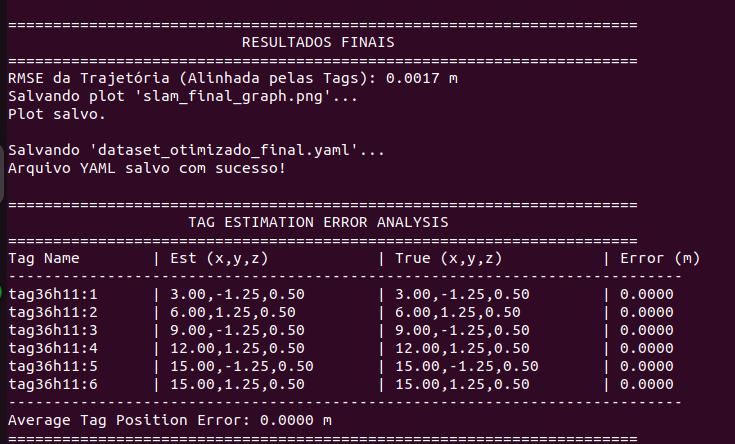
\includegraphics[width=\textwidth]{assets/straight_otmires.png}
            \vspace{0.15cm}
            {\tiny\textit{Clean dataset — straight trajectory}}
        \end{column}
        \begin{column}{0.48\textwidth}
            \centering
            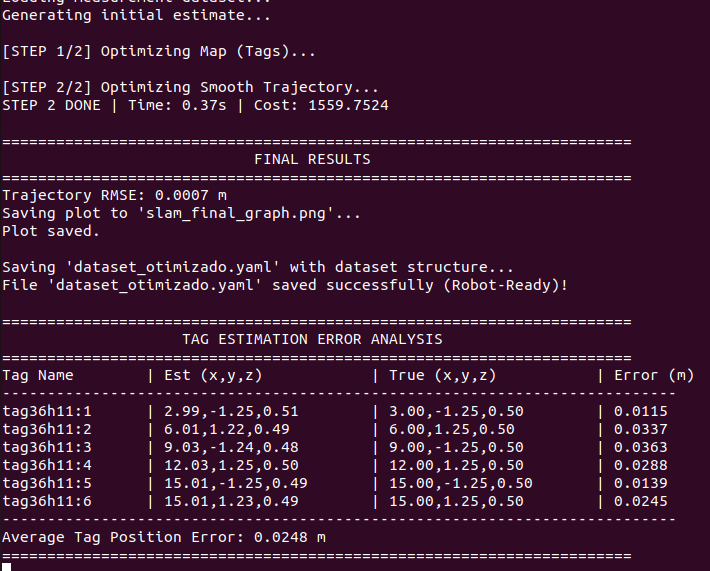
\includegraphics[width=\textwidth]{assets/straight_noisy_otmires.png}
            \vspace{0.15cm}
            {\tiny\textit{Noisy dataset — straight trajectory}}
        \end{column}
    \end{columns}
\end{frame}


\begin{frame}{Rubber duck check — S curve with 5 tags}
    \centering
    \textbf{Pato de borracha:} explico que só há ruído extra, a geometria da curva precisa continuar igual nos dois gráficos.
    \vspace{0.35cm}

    \begin{columns}
        \begin{column}{0.48\textwidth}
            \centering
            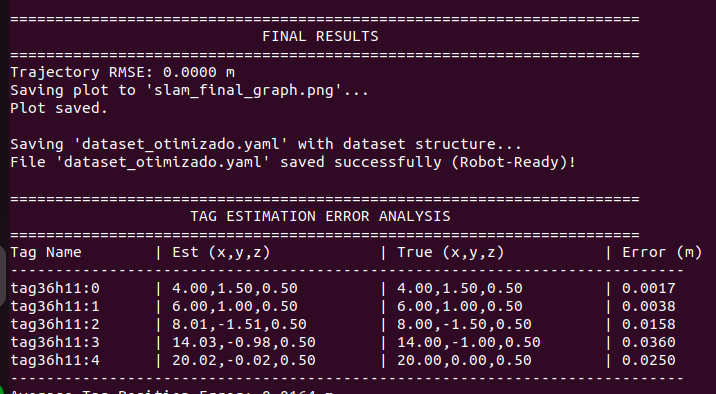
\includegraphics[width=\textwidth]{assets/s_curve_otmires.png}
            \vspace{0.15cm}
            {\tiny\textit{Clean dataset — S curve, 5 tags}}
        \end{column}
        \begin{column}{0.48\textwidth}
            \centering
            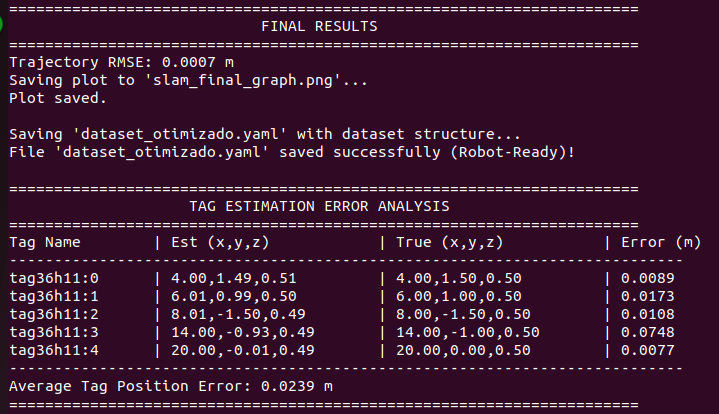
\includegraphics[width=\textwidth]{assets/s_curve_noisy_otmires.png}
            \vspace{0.15cm}
            {\tiny\textit{Noisy dataset — S curve, 5 tags}}
        \end{column}
    \end{columns}
\end{frame}


\begin{frame}{Rubber duck check — S curve with 22 tags}
    \centering
    \textbf{Pato de borracha:} mais tags para o pato conferir que densidade de medições muda, mas o caminho base permanece.
    \vspace{0.35cm}

    \begin{columns}
        \begin{column}{0.48\textwidth}
            \centering
            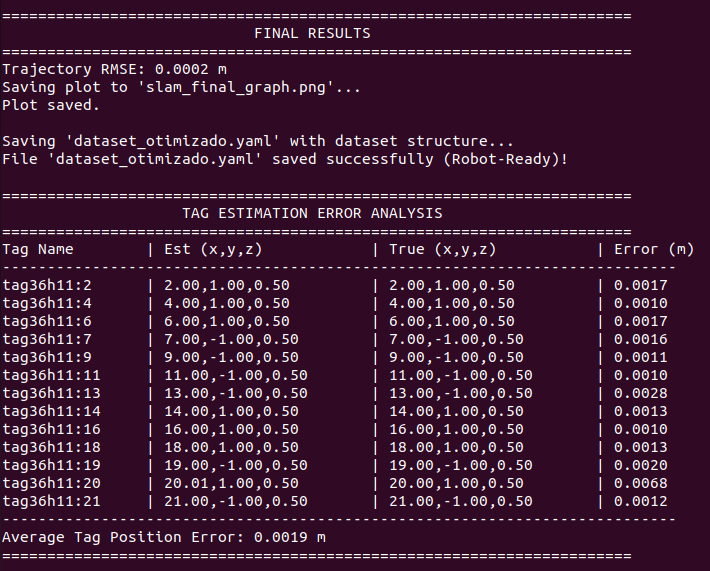
\includegraphics[width=\textwidth]{assets/s_20tags_curve_otmires.png}
            \vspace{0.15cm}
            {\tiny\textit{Clean dataset — S curve, 22 tags}}
        \end{column}
        \begin{column}{0.48\textwidth}
            \centering
            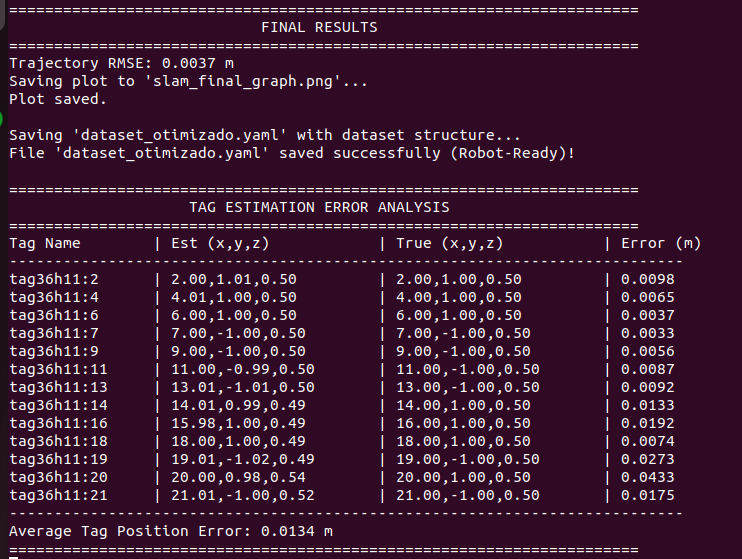
\includegraphics[width=\textwidth]{assets/s_20tags_curve_noisy_otmires.png}
            \vspace{0.15cm}
            {\tiny\textit{Noisy dataset — S curve, 22 tags}}
        \end{column}
    \end{columns}
\end{frame}

% ==================/// PHASE 5 ///==================
\begin{frame}{Phase 5: Path recovery algorithm}
    \begin{columns}
        \begin{column}{0.6\textwidth}
            \textbf{Goal: Recover when the robot leaves the taught path}
            \vspace{0.5cm}
            \begin{itemize}
                \item<1-> \textbf{Recovery logic:}  
                Simple rules to steer back to the recorded path.

                \item<2-> \textbf{Closest waypoint search:}  
                Use a quick KD-Tree to find the nearest waypoint.

                \item<4-> \textbf{Safety validation:}  
                Test recovery moves in sim to avoid bad turns.
            \end{itemize}
        \end{column}
        
        \begin{column}{0.50\textwidth}
            \centering
            \only<3->{
                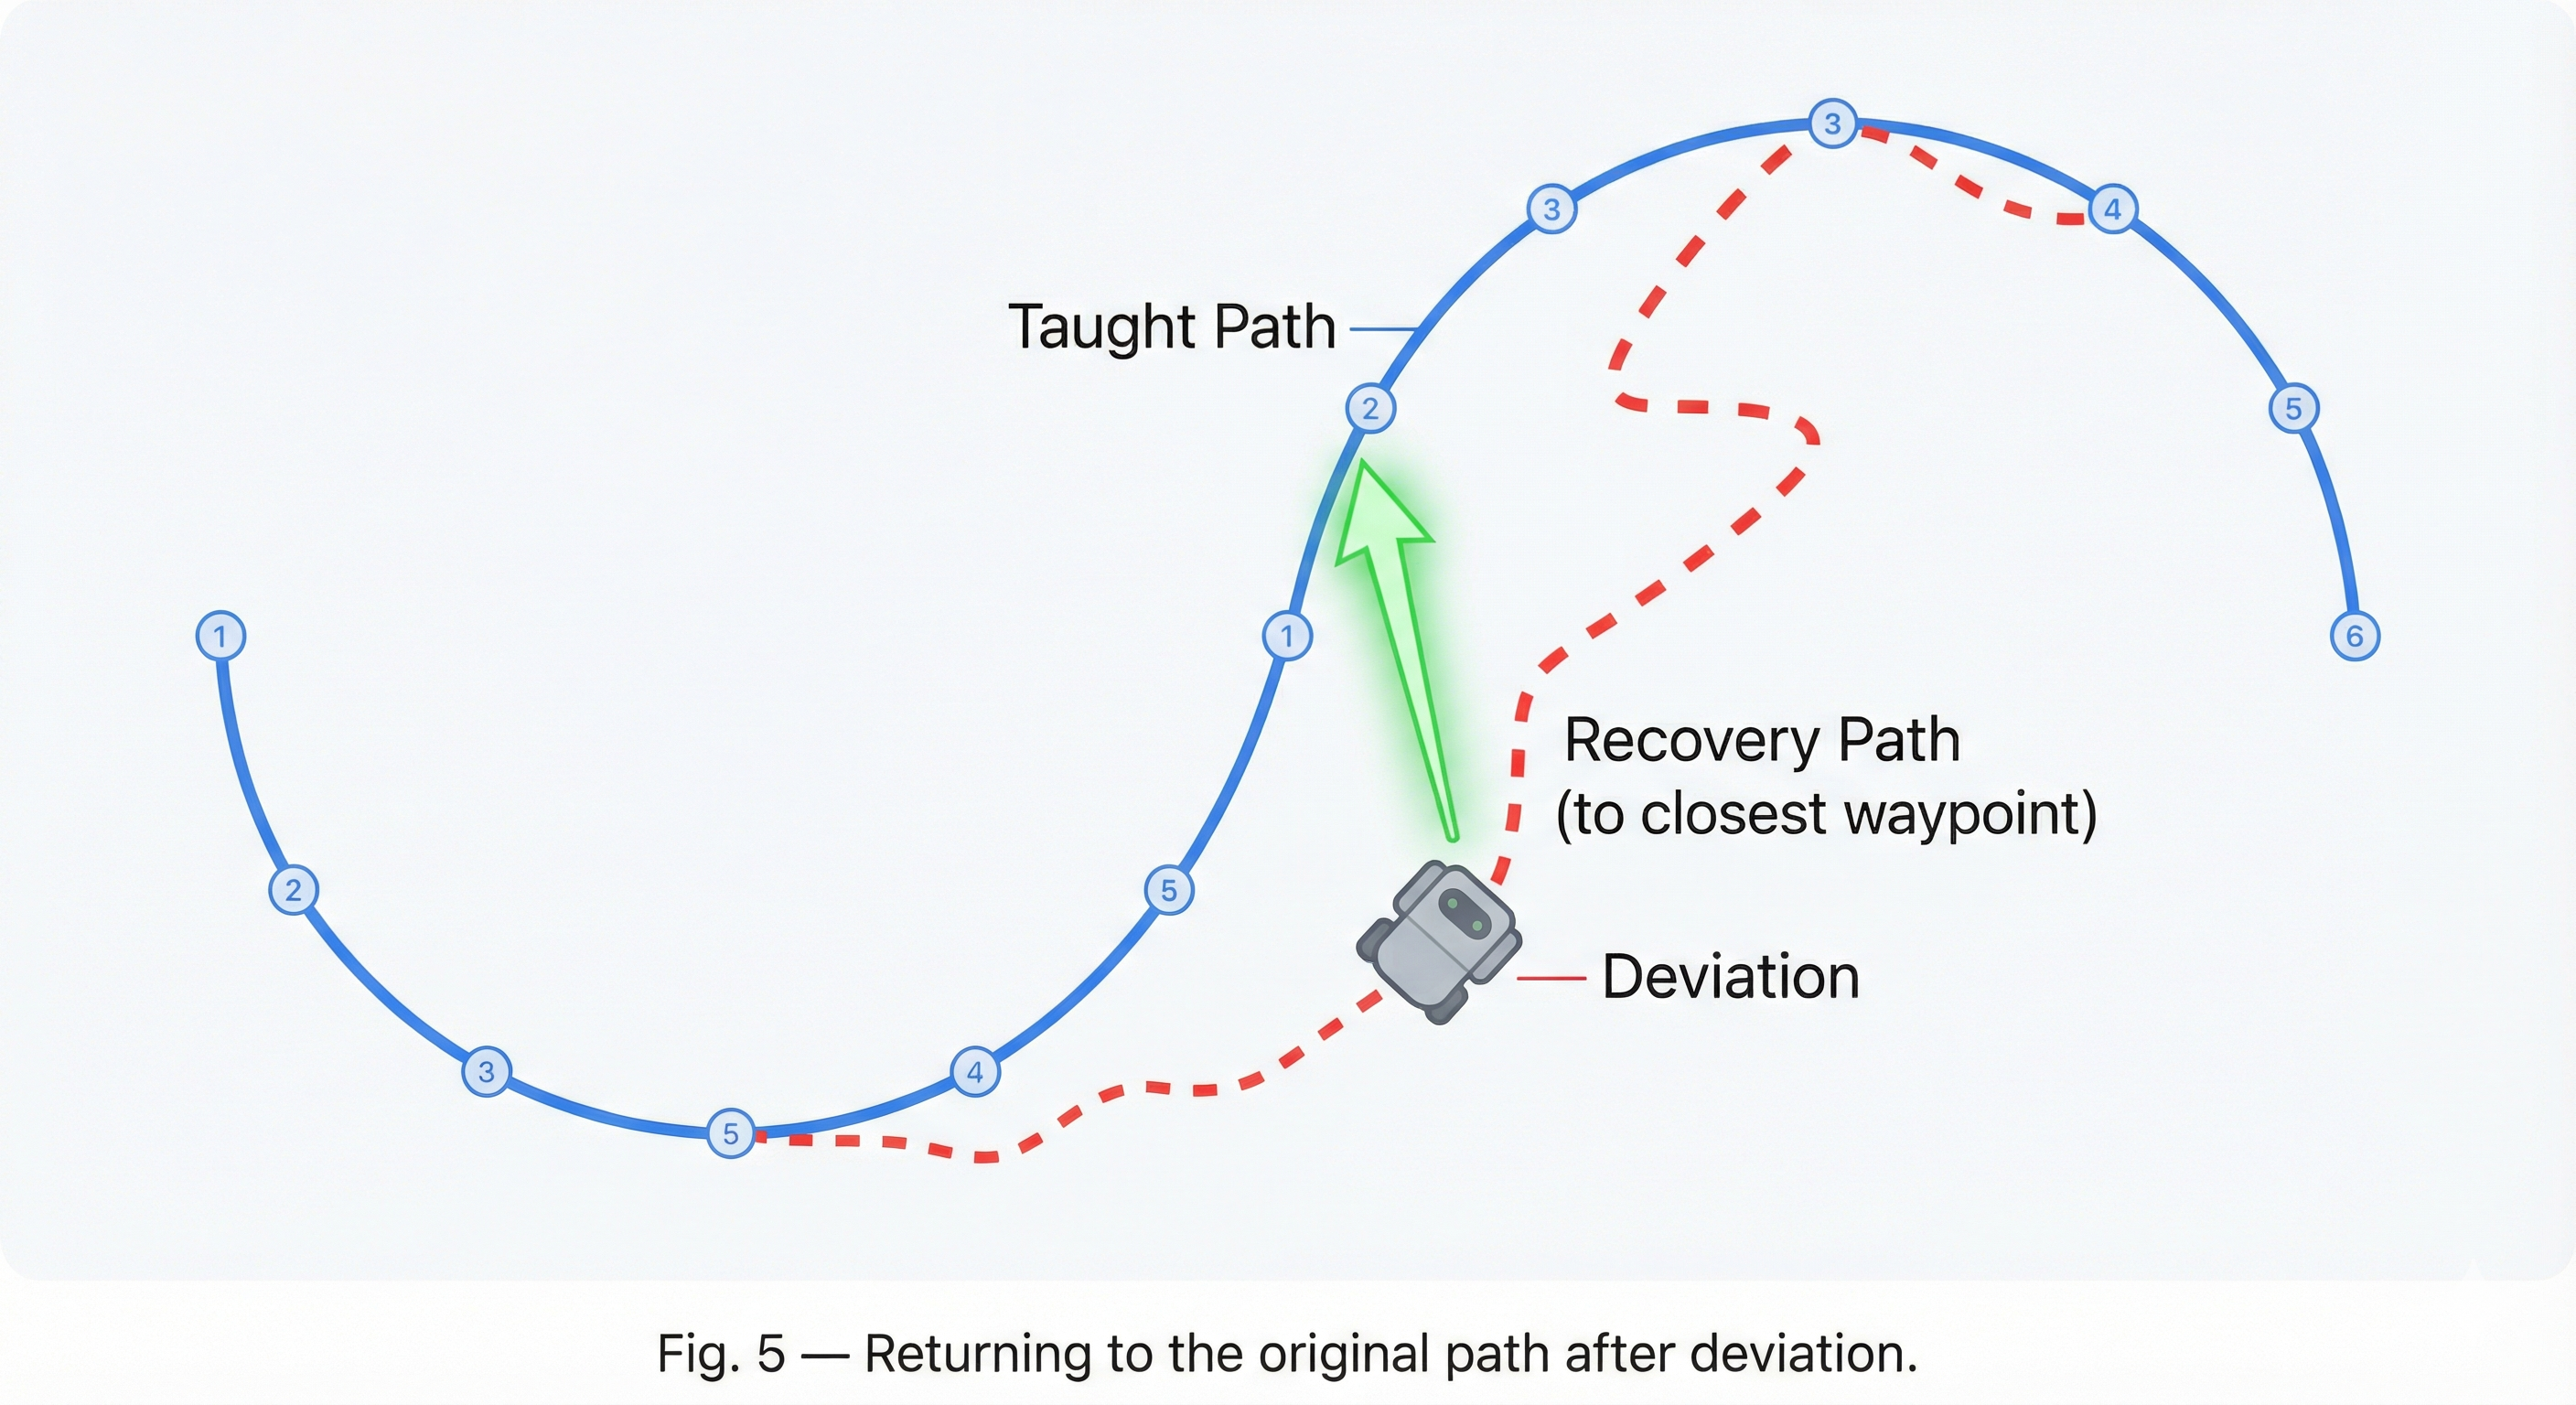
\includegraphics[trim={5cm 4cm 5cm 3cm}, clip, width=\textwidth]{assets/return_path.png}

                \vspace{0.2cm}
                {\tiny\textit{Fig. 10 — Returning to the original path after deviation}}
            }
        \end{column}
    \end{columns}
\end{frame}



% ==================/// PHASE 6 ///==================
\begin{frame}{Phase 6: System integration}
    \begin{columns}
        \begin{column}{0.6\textwidth}
            \textbf{Goal: Demonstrate full teach and repeat autonomy}
            \vspace{0.5cm}
            \begin{itemize}
                \item<1-> \textbf{Controller integration:}  
                Mix Pure Pursuit with the perception and pose stack.

                \item<2-> \textbf{Autonomous replay:}  
                Let the robot drive the recorded path on its own.

                \item<4-> \textbf{Final system:}  
                A teach \& repeat pipeline anyone can run without coding.
            \end{itemize}
        \end{column}
        
        \begin{column}{0.45\textwidth}
            \centering
            \only<3->{
                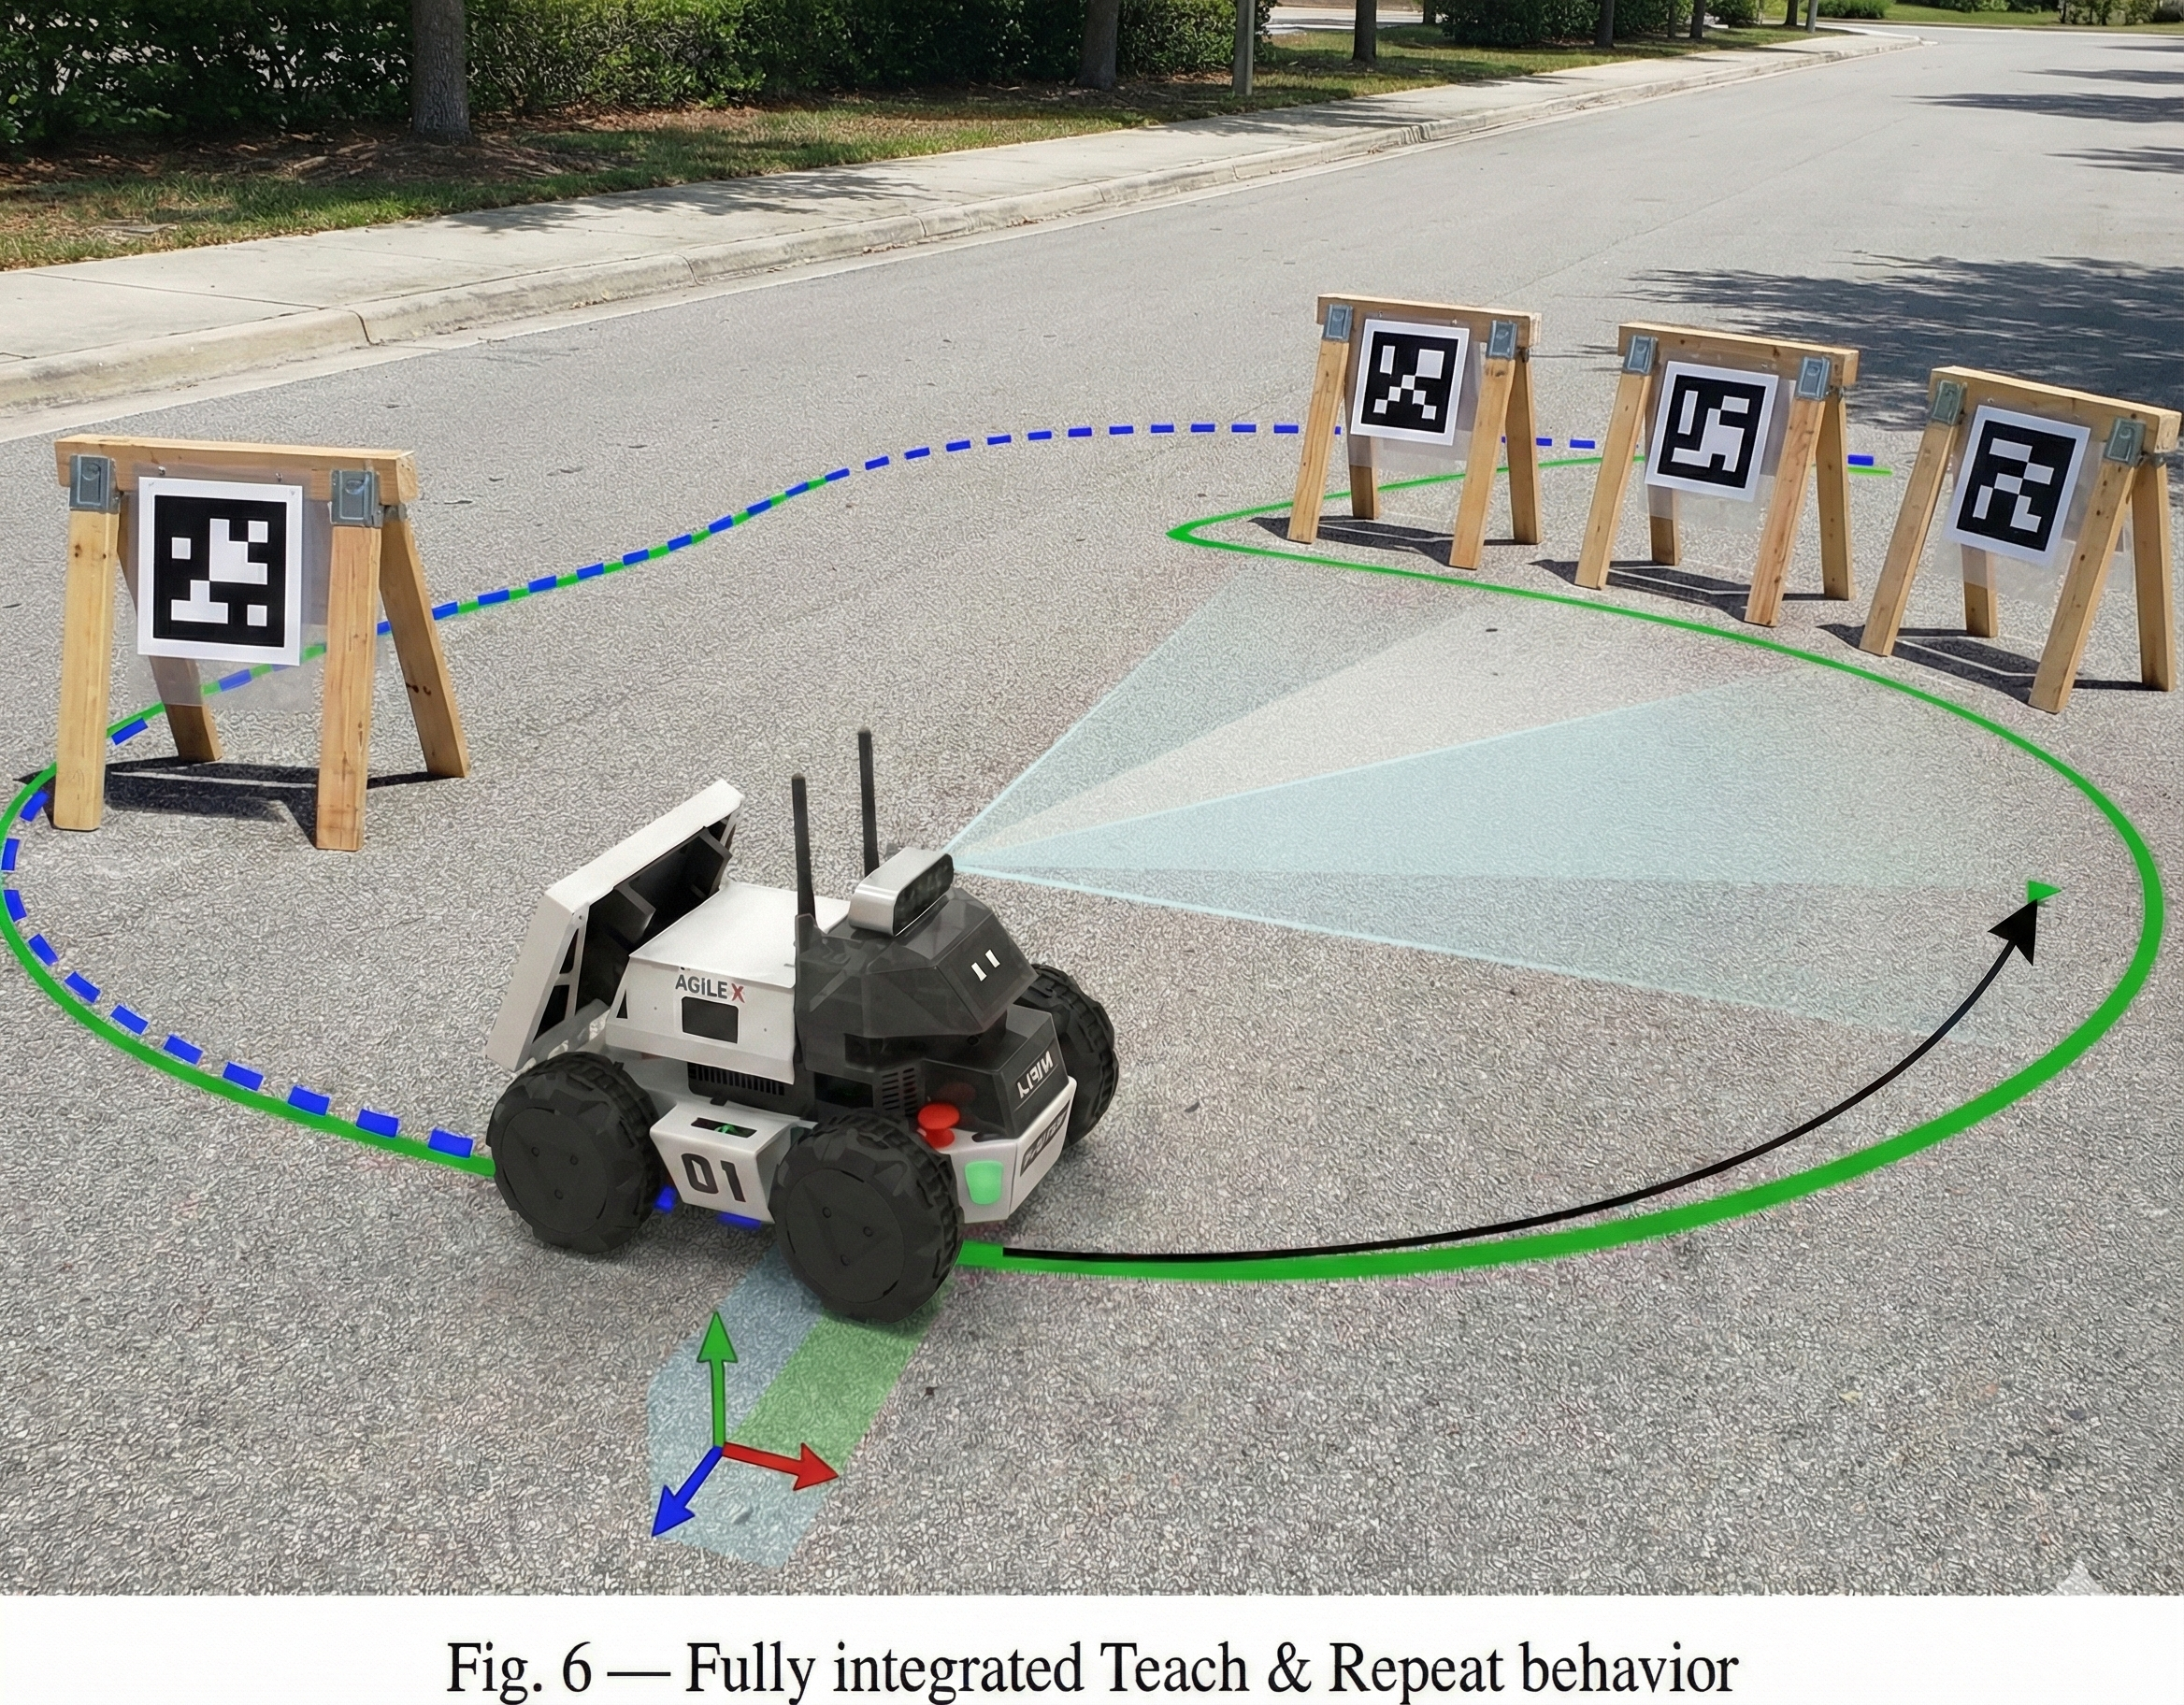
\includegraphics[trim={1cm 5cm 1cm 1cm}, clip, width=\textwidth]{assets/robot_transit.png}

                \vspace{0.2cm}
                {\tiny\textit{Fig. 11 — Fully integrated teach and repeat behavior}}
            }
        \end{column}
    \end{columns}
\end{frame}
